% Options for packages loaded elsewhere
% Options for packages loaded elsewhere
\PassOptionsToPackage{unicode}{hyperref}
\PassOptionsToPackage{hyphens}{url}
\PassOptionsToPackage{dvipsnames,svgnames,x11names}{xcolor}
%
\documentclass[
  french,
  11pt,
  a4paper,
]{report}
\usepackage{xcolor}
\usepackage[top=1.5cm, bottom=1.5cm, left=2.5cm, right=2.5cm]{geometry}
\usepackage{amsmath,amssymb}
\setcounter{secnumdepth}{-\maxdimen} % remove section numbering
\usepackage{iftex}
\ifPDFTeX
  \usepackage[T1]{fontenc}
  \usepackage[utf8]{inputenc}
  \usepackage{textcomp} % provide euro and other symbols
\else % if luatex or xetex
  \usepackage{unicode-math} % this also loads fontspec
  \defaultfontfeatures{Scale=MatchLowercase}
  \defaultfontfeatures[\rmfamily]{Ligatures=TeX,Scale=1}
\fi
\usepackage{lmodern}
\ifPDFTeX\else
  % xetex/luatex font selection
  \setmainfont[]{TeX Gyre Termes}
\fi
% Use upquote if available, for straight quotes in verbatim environments
\IfFileExists{upquote.sty}{\usepackage{upquote}}{}
\IfFileExists{microtype.sty}{% use microtype if available
  \usepackage[]{microtype}
  \UseMicrotypeSet[protrusion]{basicmath} % disable protrusion for tt fonts
}{}
\makeatletter
\@ifundefined{KOMAClassName}{% if non-KOMA class
  \IfFileExists{parskip.sty}{%
    \usepackage{parskip}
  }{% else
    \setlength{\parindent}{0pt}
    \setlength{\parskip}{6pt plus 2pt minus 1pt}}
}{% if KOMA class
  \KOMAoptions{parskip=half}}
\makeatother
% Make \paragraph and \subparagraph free-standing
\makeatletter
\ifx\paragraph\undefined\else
  \let\oldparagraph\paragraph
  \renewcommand{\paragraph}{
    \@ifstar
      \xxxParagraphStar
      \xxxParagraphNoStar
  }
  \newcommand{\xxxParagraphStar}[1]{\oldparagraph*{#1}\mbox{}}
  \newcommand{\xxxParagraphNoStar}[1]{\oldparagraph{#1}\mbox{}}
\fi
\ifx\subparagraph\undefined\else
  \let\oldsubparagraph\subparagraph
  \renewcommand{\subparagraph}{
    \@ifstar
      \xxxSubParagraphStar
      \xxxSubParagraphNoStar
  }
  \newcommand{\xxxSubParagraphStar}[1]{\oldsubparagraph*{#1}\mbox{}}
  \newcommand{\xxxSubParagraphNoStar}[1]{\oldsubparagraph{#1}\mbox{}}
\fi
\makeatother


\usepackage{longtable,booktabs,array}
\newcounter{none} % for unnumbered tables
\usepackage{calc} % for calculating minipage widths
% Correct order of tables after \paragraph or \subparagraph
\usepackage{etoolbox}
\makeatletter
\patchcmd\longtable{\par}{\if@noskipsec\mbox{}\fi\par}{}{}
\makeatother
% Allow footnotes in longtable head/foot
\IfFileExists{footnotehyper.sty}{\usepackage{footnotehyper}}{\usepackage{footnote}}
\makesavenoteenv{longtable}
\usepackage{graphicx}
\makeatletter
\newsavebox\pandoc@box
\newcommand*\pandocbounded[1]{% scales image to fit in text height/width
  \sbox\pandoc@box{#1}%
  \Gscale@div\@tempa{\textheight}{\dimexpr\ht\pandoc@box+\dp\pandoc@box\relax}%
  \Gscale@div\@tempb{\linewidth}{\wd\pandoc@box}%
  \ifdim\@tempb\p@<\@tempa\p@\let\@tempa\@tempb\fi% select the smaller of both
  \ifdim\@tempa\p@<\p@\scalebox{\@tempa}{\usebox\pandoc@box}%
  \else\usebox{\pandoc@box}%
  \fi%
}
% Set default figure placement to htbp
\def\fps@figure{htbp}
\makeatother


% definitions for citeproc citations
\NewDocumentCommand\citeproctext{}{}
\NewDocumentCommand\citeproc{mm}{%
  \begingroup\def\citeproctext{#2}\cite{#1}\endgroup}
\makeatletter
 % allow citations to break across lines
 \let\@cite@ofmt\@firstofone
 % avoid brackets around text for \cite:
 \def\@biblabel#1{}
 \def\@cite#1#2{{#1\if@tempswa , #2\fi}}
\makeatother
\newlength{\cslhangindent}
\setlength{\cslhangindent}{1.5em}
\newlength{\csllabelwidth}
\setlength{\csllabelwidth}{3em}
\newenvironment{CSLReferences}[2] % #1 hanging-indent, #2 entry-spacing
 {\begin{list}{}{%
  \setlength{\itemindent}{0pt}
  \setlength{\leftmargin}{0pt}
  \setlength{\parsep}{0pt}
  % turn on hanging indent if param 1 is 1
  \ifodd #1
   \setlength{\leftmargin}{\cslhangindent}
   \setlength{\itemindent}{-1\cslhangindent}
  \fi
  % set entry spacing
  \setlength{\itemsep}{#2\baselineskip}}}
 {\end{list}}
\usepackage{calc}
\newcommand{\CSLBlock}[1]{\hfill\break\parbox[t]{\linewidth}{\strut\ignorespaces#1\strut}}
\newcommand{\CSLLeftMargin}[1]{\parbox[t]{\csllabelwidth}{\strut#1\strut}}
\newcommand{\CSLRightInline}[1]{\parbox[t]{\linewidth - \csllabelwidth}{\strut#1\strut}}
\newcommand{\CSLIndent}[1]{\hspace{\cslhangindent}#1}

\ifLuaTeX
\usepackage[bidi=basic,shorthands=off]{babel}
\else
\usepackage[bidi=default,shorthands=off]{babel}
\fi
\ifPDFTeX
\else
\babelfont{rm}[]{TeX Gyre Termes}
\fi
\ifLuaTeX
  \usepackage{selnolig} % disable illegal ligatures
\fi


\setlength{\emergencystretch}{3em} % prevent overfull lines

\providecommand{\tightlist}{%
  \setlength{\itemsep}{0pt}\setlength{\parskip}{0pt}}



 


\usepackage{booktabs}
\usepackage{longtable}
\usepackage{array}
\usepackage{multirow}
\usepackage{wrapfig}
\usepackage{float}
\usepackage{colortbl}
\usepackage{pdflscape}
\usepackage{tabu}
\usepackage{threeparttable}
\usepackage{threeparttablex}
\usepackage[normalem]{ulem}
\usepackage{makecell}
\usepackage{xcolor}
\usepackage{caption}
\usepackage{anyfontsize}
\usepackage{enumitem}
\setlist[itemize]{label=$\bullet$}  % Puce ronde classique
\makeatletter
\@ifpackageloaded{caption}{}{\usepackage{caption}}
\AtBeginDocument{%
\ifdefined\contentsname
  \renewcommand*\contentsname{Table des matières}
\else
  \newcommand\contentsname{Table des matières}
\fi
\ifdefined\listfigurename
  \renewcommand*\listfigurename{Liste des Figures}
\else
  \newcommand\listfigurename{Liste des Figures}
\fi
\ifdefined\listtablename
  \renewcommand*\listtablename{Liste des Tables}
\else
  \newcommand\listtablename{Liste des Tables}
\fi
\ifdefined\figurename
  \renewcommand*\figurename{Figure}
\else
  \newcommand\figurename{Figure}
\fi
\ifdefined\tablename
  \renewcommand*\tablename{Table}
\else
  \newcommand\tablename{Table}
\fi
}
\@ifpackageloaded{float}{}{\usepackage{float}}
\floatstyle{ruled}
\@ifundefined{c@chapter}{\newfloat{codelisting}{h}{lop}}{\newfloat{codelisting}{h}{lop}[chapter]}
\floatname{codelisting}{Listing}
\newcommand*\listoflistings{\listof{codelisting}{Liste des Listings}}
\makeatother
\makeatletter
\makeatother
\makeatletter
\@ifpackageloaded{caption}{}{\usepackage{caption}}
\@ifpackageloaded{subcaption}{}{\usepackage{subcaption}}
\makeatother
\usepackage{bookmark}
\IfFileExists{xurl.sty}{\usepackage{xurl}}{} % add URL line breaks if available
\urlstyle{same}
\hypersetup{
  pdflang={fr},
  colorlinks=true,
  linkcolor={blue},
  filecolor={Maroon},
  citecolor={Blue},
  urlcolor={Blue},
  pdfcreator={LaTeX via pandoc}}


\author{}
\date{}
\begin{document}


\begin{titlepage}
\centering


\includegraphics{ensai_logo_1.png}\\
\vspace{1.0cm}

{\LARGE\textsc{Rapport de Projet statistique}}\\
\vspace{0.5cm}
{\large Élèves 1A}
{\large Groupe 15}

\vspace{2.5cm}

\rule{\textwidth}{0.5mm}\\
\vspace{0.8cm}
{\huge\bfseries Inégalité de niveau scolaire dans les pays de l’OCDE}\\
\vspace{0.8cm}
\rule{\textwidth}{0.5mm}\\

\vspace{2.5cm}

\begin{flushleft}
\emph{Étudiant·e·s :}\\
Torreilles Raphaël \\
Delanzy Romane \\
Blanc Benjamin \\
\end{flushleft}

\begin{flushright}
\emph{Responsable :}\\
Laurent COSTA\\
\vspace{1.0cm}
\emph{Encadrant(e) :}\\
Louis GERVILLE-REACHE\\
\end{flushright}

\vfill 
\begin{center}
École nationale de la statistique et de l’analyse de l’information\\
2025--2026
\end{center}
\end{titlepage}

\tableofcontents

\chapter{Introduction}\label{introduction}

Depuis 1948, l'Organisation des Nations Unies considère l'accès à
l'éducation comme un droit. Considérée comme un pilier des sociétés
démocratiques, l'école à vocation à garantir l'égalité des chances en
offrant à chaque enfant quelque soit son origine sociale, son
environnement familial ou encore son lieu de naissance l'accès au même
enseignement. On souhaite que ce lieu incarne la méritocratie,
c'est-à-dire un lieu où le mérite et le travail doivent primer sur le
capital économique, social et familial.

Pourtant, la plupart des études empiriques montrent le contraire.
L'école ne réduit pas les inégalités, elles les cristallisent. D'après
une étude de l'INSEE, en France, en 2022, un enfant de cadre à quatre
fois plus de chance d'obtenir un diplôme du supérieur qu'un enfant
d'ouvrier. En effet, les performances scolaires sont guidées en grande
partie par les caractéristiques individuelles. L'origine sociale, le
niveau de revenu des familles, le genre ou encore le parcours migratoire
des élèves peuvent influencer la réussite scolaire. Ce phénomène traduit
une difficulté structurelle quant à la capacité de l'école à garantir
l'égalité des chances.

Afin de mesurer et comprendre ces mécanismes, le Programme International
pour le Suivi des Acquis des élèves,connu sous l'acronyme PISA
(Programme for International Student Assessment) à été créé. Lancé par
l'OCDE (Organisation de Coopération et de Développement Économiques) en
2000 et reconduit tous les trois ans, PISA permet d'évaluer les
compétences des élèves de 15 ans dans trois domaines fondamentaux : les
mathématiques, la lecture et les sciences. En 2022, cette enquête a
mobilisé 690 000 élèves dans 81 pays. De par son nombre et la diversité
de questions posées, elle permet de croiser de nombreuses dimensions
telles que le niveau de performance académique, le statut
socio-économique et culturel de la famille, les conditions
d'enseignement, et les caractéristiques individuelles de l'élève. Elle
offre ainsi une lecture multidimensionnelle des inégalités scolaires, à
une échelle internationale.

C'est de cette enquête qu'est issue la base de données que nous allons
utiliser dans ce rapport. Nous disposons alors d'un certain nombre de
variables quant aux caractéristiques socio-économiques, familiales et
sociétales des individus ainsi que des informations quant au milieu
scolaire dans lequel ils évoluent. Elle va alors nous permettre de
comprendre, comment l'école qui a vocation à permettre à tous de
réussir, n'est souvent considérée que comme multiplicateur des
inégalités de départ. Il existe, selon de nombreux auteurs tel que
Bourdieu, qui affirmait que le système scolaire contribue à la
reproduction des inégalités (la Reproduction 1970) des facteurs
favorisant la réussite scolaire. Cependant, nous pouvons nous demander
si ces facteurs diffèrent selon les pays ou selon les individus. De même
si certains facteurs favorisent toujours la réussite scolaire, sont-ils
toujours combinés avec les mêmes facteurs ? Leur contribution était
toujours aussi importante selon les autres caractéristiques des
individus ?

Ainsi la question suivante semble émerger : \textbf{Les sources des
inégalités de niveau scolaire dans les pays de l'OCDE sont-elles les
mêmes à l'échelle individuelle qu'à l'échelle nationale ?}

Pour répondre à cette problématique nous avons fait le choix de nous
intéresser en premier lieu aux sources des inégalités scolaire dans les
pays de l'OCDE à l'échelle de chaque individu. En second lieu, nous
cherchons à comprendre les facteurs d'inégalités scolaires au niveau
individuel sont les mêmes qui favorisent la réussite d'un pays. Enfin,
nous mettrons en évidence les facteurs structurants des inégalités
scolaire grâce à une approche d'analyse en composantes principales.

\chapter{Cadrage}\label{cadrage}

Pour répondre à notre problématique, il semble primordial de mesurer le
niveau scolaire des élèves scolarisés au sein des pays de l'OCDE. Avant
toutes choses, nous avons nettoyé la base de données initiale en
retirant les données relatives à tout les pays qui ne faisaient pas
partie de l'OCDE. Quant à la mesure du niveau scolaire, nous avons fait
le choix de créer une moyenne par matière pour chaque élève. Pour ce
faire, nous avons fait la moyenne des 10 valeurs possibles
(plausible\_values) pour chaque élève par domaine. Ainsi nous avons
obtenu les variables moyenne\_lecture, la moyenne en lecture des élèves,
moyenne\_maths, la moyenne en mathématiques des élèves et
moyenne\_sciences la moyenne en sciences des élèves. Nous nous sommes
rendu compte au cours de l'analyse que les moyennes des élèves en
lecture, sciences et mathématiques étaient corrélées. Ainsi pour
simplifier le rapport et le rendre davantage compréhensible, nous avons
fait le choix de réaliser la plupart des analyses à travers la variable
moyenne\_g qui correspond à la moyenne générale des élèves (moyenne de
moyenne\_lecture, moyenne\_maths et moyenne\_sciences).

D'autre part, pour mener notre analyse, il est nécessaire de pouvoir
confronter le niveau scolaire des élèves avec différentes variables qui
les caractérisent et qui caractérisent leur environnement. Nous avons
donc sélectionné les variables qui nous semblaient être les plus
pertinentes dans la base de données initiales. Nous les avons ensuite
regroupées en trois catégories distinctes: les variables
socio-économiques, les variables socio-familiales et celles définissant
l'environnement scolaire de l'élève. Nous avons ensuite cherché à
comprendre la manière dont étaient construites ces variables.

Nous avons regroupé les individus d'un même pays dans une nouvelle base
de données niveau\_pays. Cela a été possible grace à la variable CNT qui
correspond au code ISO des pays. Cette manipulation a pour objectif
d'étudier la réussite de ces derniers à l'échelle nationale. Nous avons
ensuite regrouper ces pays en 3 groupes : les forts, les moyens et les
faibles. Pour se faire, nous avons créer la variable score\_moyen qui
correspond à la moyenne de la variable score\_global de l'ensemble des
élèves d'un même pays. Elle nous a ainsi permis de classer les pays par
niveau. Voici les groupes que nous avons obtenus. Une autre méthode
d'analyse que nous avons mis en place est de se concentrer que les 5
pays les plus performants et les 5 qui le sont le moins. Le graphique ci
dessous les mets en avant.

\begin{figure}

\centering{

\pandocbounded{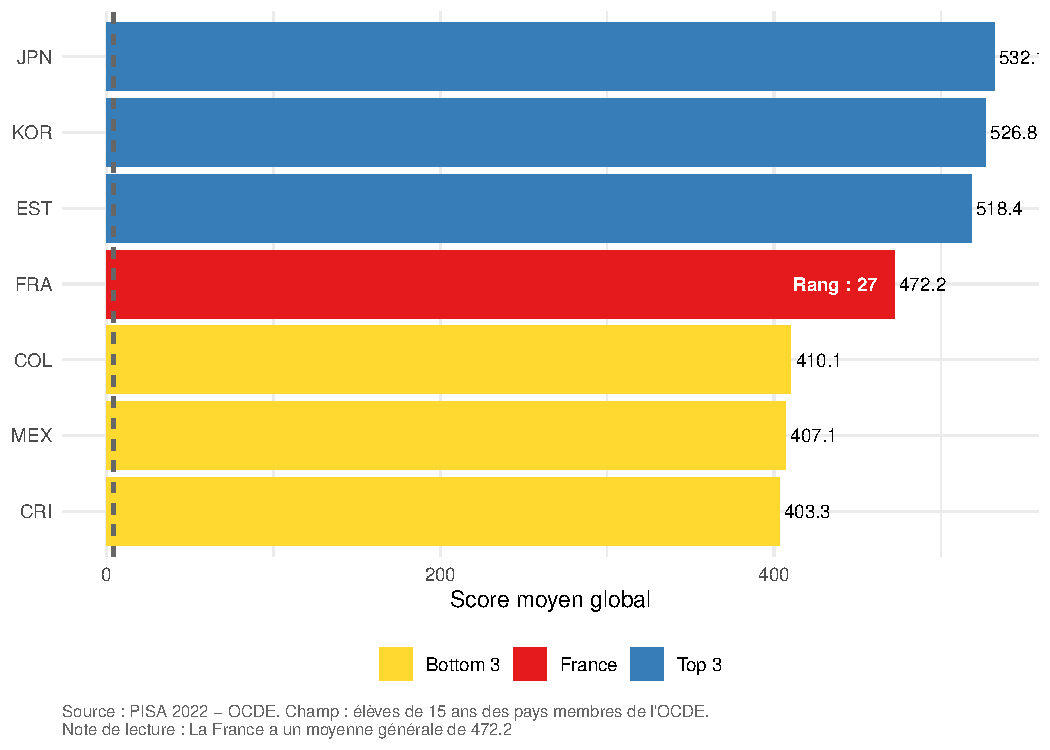
\includegraphics[keepaspectratio]{rapport_files/figure-pdf/fig-1-1.pdf}}

}

\caption{\label{fig-1}Classement des pays de l'OCDE}

\end{figure}%

Enfin, il nous semble important d'évoquer le traitement des données
manquantes. La plupart des élèves n'ont pas répondu à toutes les
questions. Nous avons choisis d'exclure un individu d'une analyse
lorsqu'il n'avait pas répondu à la question de la variable analysée,
sans l'exclure de la totalité de l'analyse. La perte d'information
aurait été trop grande. Ainsi, si un individu n'a pas renseigné de
niveau ESCS, on ne le prendra pas en compte dans l'analyse du lien entre
l'indice ESCS et le niveau scolaire. On le considèrera par contre, dans
l'analyse avec toutes les autres variables et le niveau scolaire. Ce
choix est en prendre en compte dans l'analyse. Un lien fort mais basé
sur peu de variables ne peut être interpréter de la même manière que
s'il avait été réalisé sur une variable dont aucune observation n'est
manquante. Dans le cadre de l'ACP, nous avons fait le choix de ne pas
considérer les variables PARINVOL et PQSCHOOL, plutôt que de ne pas
considérer certains individus. Ce choix sera explicité dans la partie
concernée.

\chapter{I --- Les sources des inégalités de niveau
scolaire}\label{i-les-sources-des-inuxe9galituxe9s-de-niveau-scolaire}

Au sein des pays de l'OCDE, les résultats scolaires très diversifié. Les
résulats varient d'un élève à l'autre. Les élèves ne réussissent pas
tous à obtenir les meilleures notes possibles. Nous cherchons donc à
déterminer les facteurs à l'origine des bons et mauvais résultats. Nous
allons donc étudier les liens entre les variables économiques, scolaires
et familiales et les résultats scolaire d'un élève.

\section{A --- L'influence des variables économiques sur les inégalités
de niveau
scolaire}\label{a-linfluence-des-variables-uxe9conomiques-sur-les-inuxe9galituxe9s-de-niveau-scolaire}

Lorsqu'on pense aux inégalités de niveau scolaire, on imagine comme
première cause les inégalités économiques. De nombreuses études de
l'INSEE montre que dès l'entrée à l'école les enfants issuent de milieux
sociaux favorisés ont des acquis supérieurs à ceux issuent de milieux
défavorisés. L'indice ESCS est un indice composite crée par l'OCDE afin
de mesurer le statut socio-économique d'un individu. Nous allon alors le
lien entre la réussite scolaire d'un élève et son statut
socio-économique.

\begin{verbatim}
                  [,1]
PQSCHOOL   -0.03258278
SCHSUST     0.13967888
ST127Q01TA -0.24718295
ST059Q01TA -0.05422211
ST059Q02JA  0.22097587
EXPO21ST   -0.03422120
ESCS        0.40834189
HISEI       0.35080447
HOMEPOS     0.41055076
LEARRES     0.01001788
PARINVOL   -0.18357175
\end{verbatim}

\begin{verbatim}
                  [,1]
PQSCHOOL   -0.03258278
SCHSUST     0.13967888
ST127Q01TA -0.24718295
ST059Q01TA -0.05422211
ST059Q02JA  0.22097587
EXPO21ST   -0.03422120
ESCS        0.40834189
HISEI       0.35080447
HOMEPOS     0.41055076
LEARRES     0.01001788
PARINVOL   -0.18357175
\end{verbatim}

\begin{verbatim}
           score_global
ST127Q01TA   0.25199534
PROGN        0.49172807
CNT          0.28446604
ST255Q01JA   0.46169415
FL170Q02JA   0.17392908
FL170Q03JA   0.17634483
ST294Q01JA   0.14690897
ST295Q04JA   0.22673903
ST295Q03JA   0.08849546
DURECEC      0.11318967
HISCED       0.27671638
FISCED       0.30430856
MISCED       0.27843511
IMMIG        0.09318792
ST004D01T    0.02455695
ST016Q01NA   0.24090272
ST260Q01JA   0.12957117
ST267Q02JA   0.09650753
ST295Q02JA   0.17713821
ST307Q01JA   0.18119523
WB150Q01HA   0.09347890
\end{verbatim}

Avant tout, nous nous sommes intéréssé à ce que l'on pensait être le
principal facteur d'inégalité de résultat scolaire: la situation
socio-économique de l'élève. Sur le graphique ci-dessous, on constate un
lien entre le score global de l'élève et l'indice ESCS. L'indice ESCS
(Economic, Social and Cultural Status) est un indice composite construit
par l'OCDE pour mesurer le statut socio-économique et culturel des
élèves. C'est un indice standardisé à l'échelle OCDE. Cela signifie
qu'il est construit de telle manière que sa moyenne est de 0 et son
écart-type de 1. Il est formé à partir de trois indices : le statut
socioprofessionnel des parents (HISEI), le niveau de formation (PARED)
des parents, ainsi que le patrimoine familial (HOMEPOS). Ce dernier
indice inclut lui-même un grand nombre de variables parmi lesquelles les
ressources culturelles, éducatives ainsi que d'autres ressources. On
constate, en effet, que les élèves ayant un indice ESCS plus élevé ont
tendance à avoir des meilleures notes. Ainsi, ce graphique traduit un
lien entre réussite scolaire et niveau de capital économique. Plus
l'individu est aisé, plus il a de chance de réussir à l'école. Cependant
cela ne signifie pas que toutes les variables économiques sont
impactantes quant à la réussite d'un élève. Ainsi, nous avons choisi
d'étudier un certain nombre de variables représentatives, chacune à leur
manière d'un certain capital économique.

\begin{figure}

\centering{

\pandocbounded{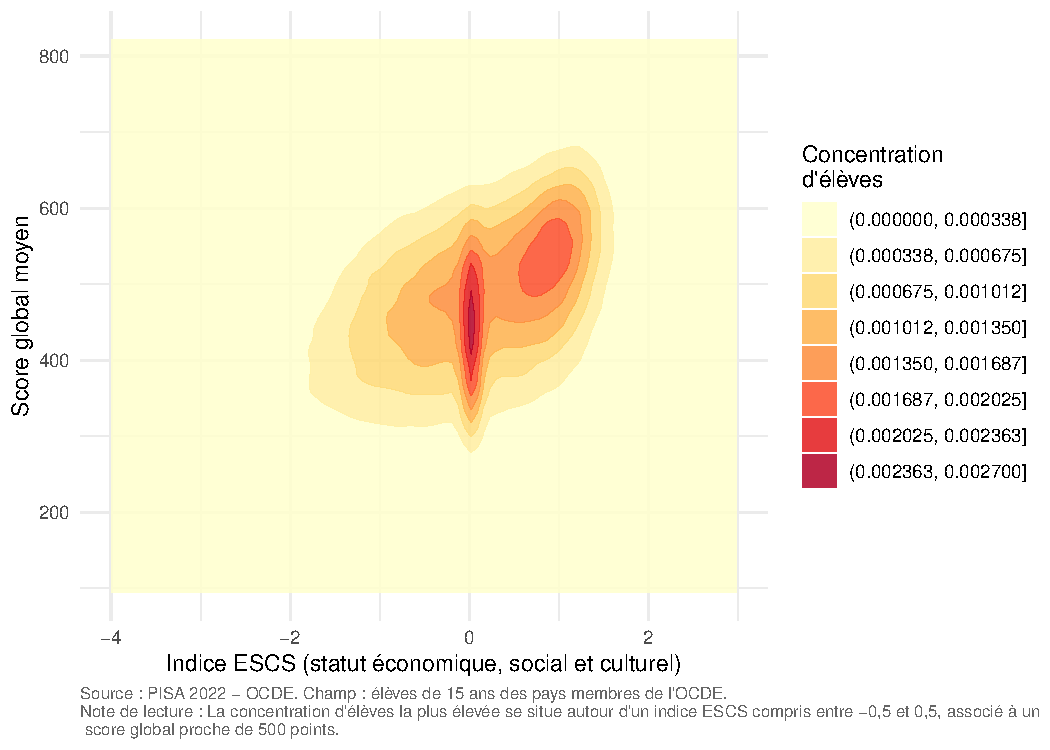
\includegraphics[keepaspectratio]{rapport_files/figure-pdf/fig-3-1.pdf}}

}

\caption{\label{fig-3}Lien entre statut socio-économique (ESCS) et score
global}

\end{figure}%

Pour étudier de manière individuelle l'impact de chaque variable de
nature économique, nous avons réalisé deux matrices de corrélation. Une
pour les variables quantitatives et une pour les variables qualitatives.
Pour les variables quantitatives nous avons utilisé le coefficient de
corrélation. Cet indicateur statistique permet de mesurer l'intensité et
le sens de la relation linéaire entre deux variables quantitatives. Il
est compris entre -1 et 1. Pour les variables qualitatives nous avons
utilisé le rapport de corrélation. Il indique quelle part de la
variation d'une variable est expliquée par une autre. Il est quant à lui
compris entre 0 et 1.

\begin{figure}

\centering{

\pandocbounded{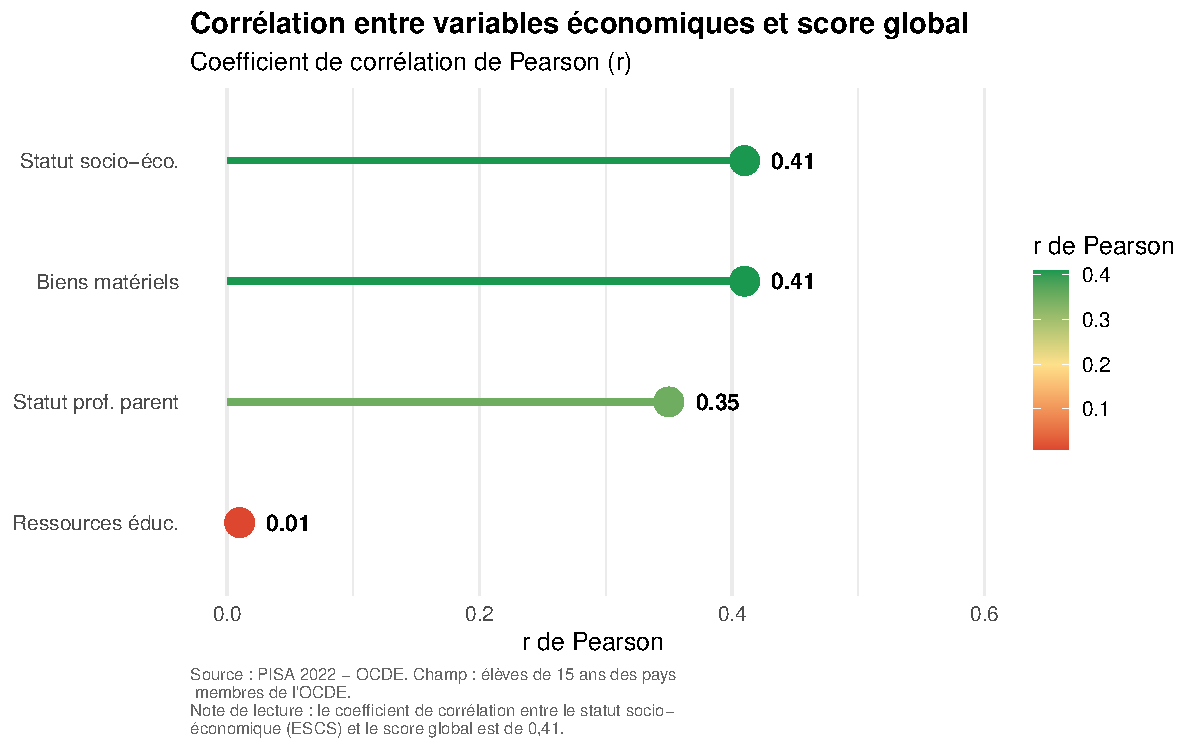
\includegraphics[keepaspectratio]{rapport_files/figure-pdf/fig-4-1.pdf}}

}

\caption{\label{fig-4}Corrélation entre variables quantitatives
économique et score global}

\end{figure}%

\begin{figure}

\centering{

\pandocbounded{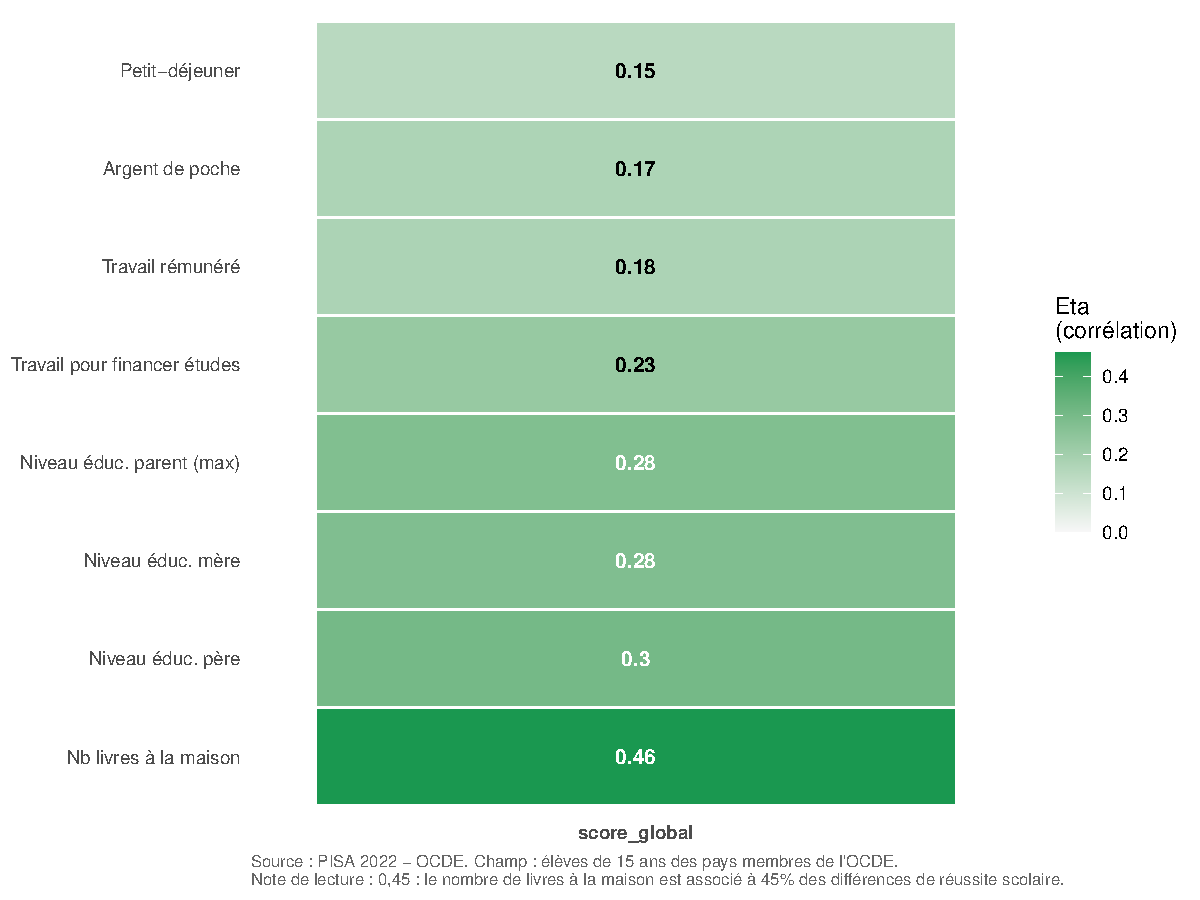
\includegraphics[keepaspectratio]{rapport_files/figure-pdf/fig-5-1.pdf}}

}

\caption{\label{fig-5}Force du lien entre variables qualitatives de
nature économique et scores scolaires}

\end{figure}%

Dans un premier temps, on constate le statut professionnel des parents
ainsi que la possession de biens matériels sont également corrélés au
niveau scolaire. Cela s'explique simplement par le fait que l'indice
ESCS est composé des indices HOMEPOS et HISEI. Au delà de ce simple fait
statistique, on peut facilement penser que la profession des parents
impactent celle des enfants. Un effet de reproduction sociale se met en
place. Un parent ayant fait de longue étude aura souvent tendance à
pousser son enfant à faire de même.

Au delà de cet indice, un autre lien important semble émerger. Plus un
enfant a de livres chez lui plus il réussit à l'école. On considère dans
cette partie de l'analyse que possèder des livres en quantité importante
est lié au capital économique. Cette hypothèse est vérifiée par les
chiffres puisque le coefficient entre l'indice ESCS et ST255Q01JA est de
0,5. Plus une famille est aisé plus elle détient le pouvoir d'achat
nécessaire pour acheter des livres en quantité importante. Ainsi on peut
considérer la possession de livre comme signe de richesse. Possèder des
livres peut pour un enfant, faciliter l'apprentissage de discipline
fondamentale comme la lecture et éveiller l'esprit des
enfants.Cependant, une famille moins aisé peut également posséder des
livres en quantité importante. On étudiera ce point dans la partie sur
les caractéristiques socio-familiale.

D'autre part, on constate que la présence de ressources éducatives lors
de période de fermeture d'école est indépendante de la réussite
scolaire. On pourrait penser qu'un enfant possédant davantage de
ressources peut en bénéficier lors de son apprentissage en dehors du
temps scolaire favorisant ainsi sa réussite. Pourtant les chiffres nous
démontrent le contraire. Posséder des ressources éducatives
n'influencent pas la réussite scolaire. On peut alors supposer que la
plus part de l'apprentissage se fait lors du temps scolaire ou encore
que la présence de ressources éducatives au domicile familial s'il n'est
pas associé à des compétences d'enseignement n'est que peu utile.

Quant aux autres variables de nature économiques,leur effet quant à
l'explication des inégalités de niveau scolaire reste modéré. Nous en
pouvons donc ni en conclure un véritable lien significatif ni en
conclure une absence de lien.

Finalement, les inégalités économiques sont liées aux inégalités de
niveau scolaire. L'indice de statut économoque est social est corrélé au
niveau scolaire. Le statut socio-professionnel des parents et les
possesions de biens matériels qui composent cet indice le sont aussi. La
possesion de livres est également lié au niveau scolaire alors que les
ressources à disposition de l'élève lors de fermeture d'école est
indépendante de sa réussite.

\section{B --- L'environnement scolaire est-il vecteur des inégalités de
niveau
scolaire}\label{b-lenvironnement-scolaire-est-il-vecteur-des-inuxe9galituxe9s-de-niveau-scolaire}

Au sein des pays de l'OCDE, il existe une grande diversité de systèmes
éducatifs. La plupart des pays ont un fonctionnement unique qui diffère
par les horaires d'enseignement, l'importance relative des matières ou
encore par la pratique ou non du redoublement. Au sein d'un même pays,
un certain nombre de caractéristiques restent relatives à
l'établissement en lui-même ou aux professeurs qui y enseignent. Ainsi,
la scolarité de chaque élève diffère selon le pays où il étudie et les
établissements qu'il fréquente. Nous cherchons alors dans cette partie à
savoir si cette différence de système éducatif et de professeurs qu'aura
l'élève au cours de sa scolarité auront un impact sur sa réussite
scolaire. Un certain nombre de variables nous permet d'étudier cet
impact. Nous disposons notamment dans le cadre de l'enquête PISA les
variables suivantes: PQ SCHOOL qui représente la qualité de
l'établissement scolaire, SCHSUST représentant les actions de
l'établissement pour soutenir les apprentissages, ST272Q01JA à propos de
la qualité d'enseignement des mathématiques. Ces variables vont nous
permettre d'en apprendre davantage sur l'impact de la qualité des
établissements sur le niveau scolaire des élèves. Nous disposons
également de variables décrivant l'environnement scolaire national afin
d'en étudier encore une fois l'impact sur la réussite scolaire. Nous
avons ST059Q01TA à propos du nombre d'heure de mathématiques par
semaine, ST059Q02J représentant le nombre total d'heures de cours par
semaine, ainsi que EXPO21ST pour l'exposition aux mathématiques du XXIe
siècle et enfin PROGN pour Programme national d'études.

Nous nous intéressons premièrement aux variables liées aux
établissements scolaires. Le coefficient de corrélation de Pearson (r)
quantifie l'intensité et le sens du lien linéaire entre deux variables
quantitatives.

\begin{figure}

\centering{

\pandocbounded{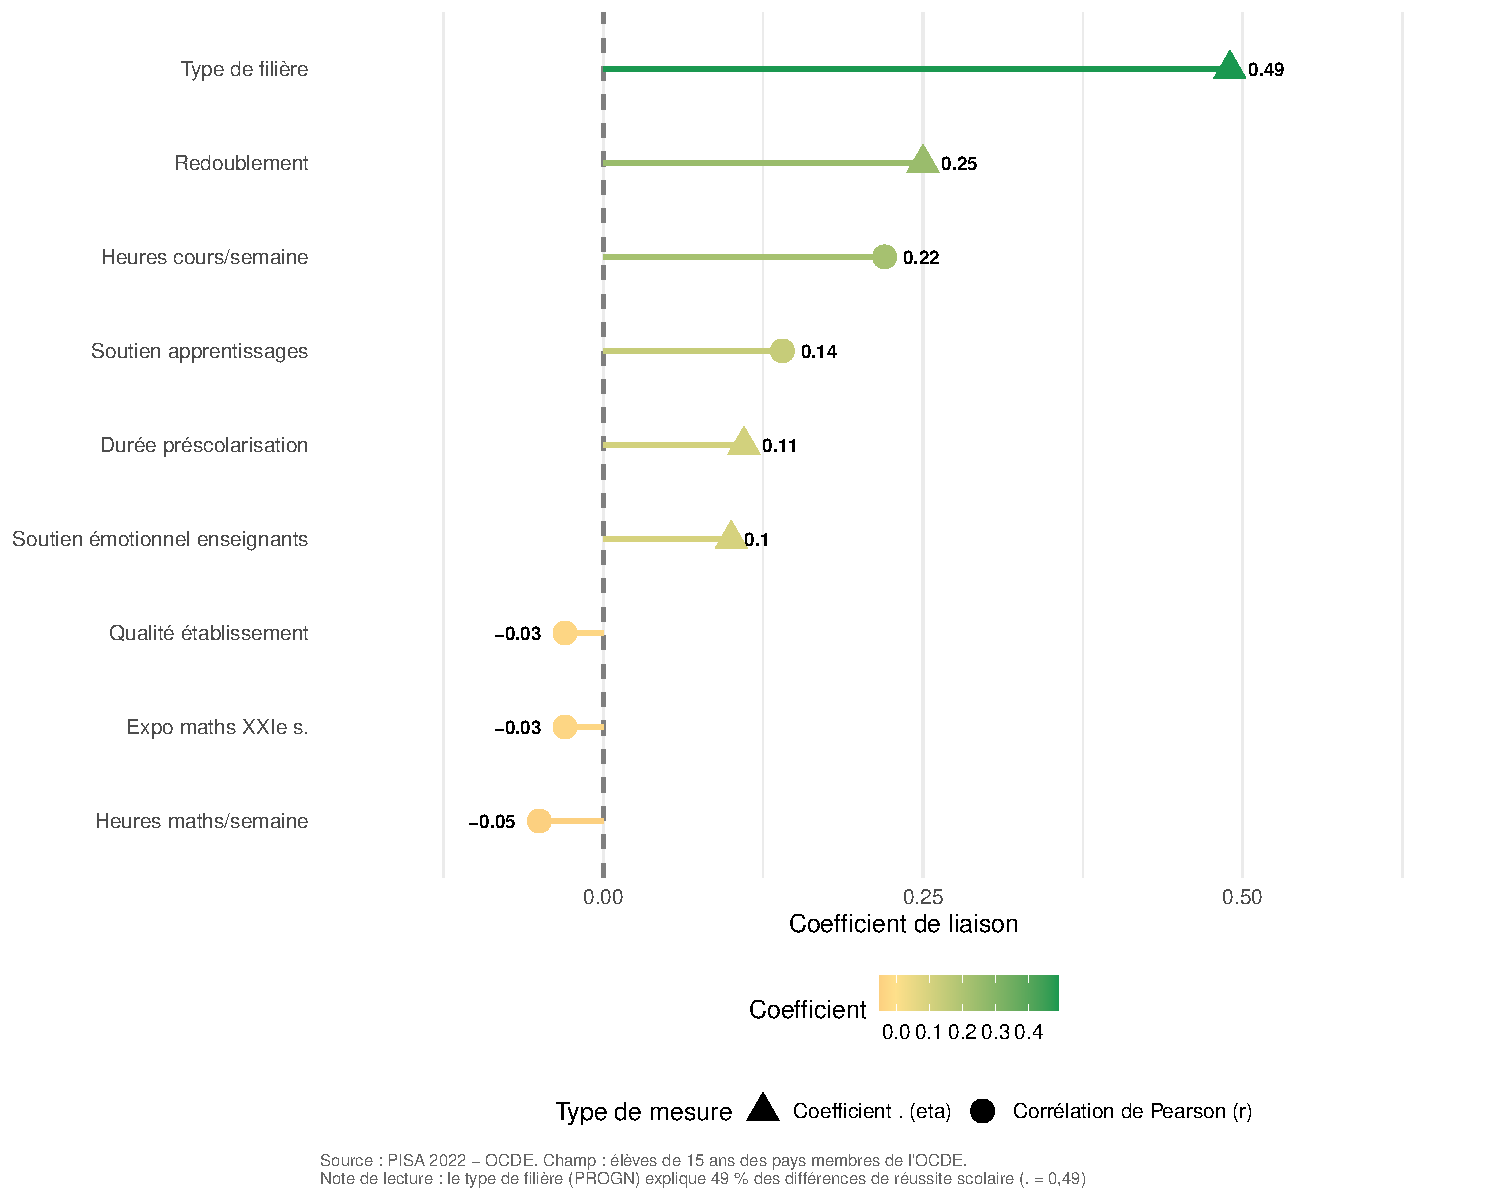
\includegraphics[keepaspectratio]{rapport_files/figure-pdf/fig-8-1.pdf}}

}

\caption{\label{fig-8}Variables scolaires et lien avec le score global}

\end{figure}%

On constate sur le tableau des corrélations ci-dessus une relation quasi
nulle entre la qualité perçue de l'établissement (PQSCHOOL) et les
scores scolaires ce qui suggère l'absence de lien linéaire entre ces
deux variables. Avant d'essayer d'analyser ce résultat, il est important
de noter que cette variable a un taux de non-réponse de plus de 80\%.
Ainsi, cette absence de lien peut être du à un taux de réponse trop
faible. Passant au delà du manque de réponse, on pourrait penser qu'une
bonne qualité d'enseignement favorise la réussite scolaire. Or le
coefficient de corrélation est bien trop proche de 0 pour en déduire
quoi que ce soit. Ainsi il est davantage pertinent de dire qu'il n'y a
pas de corrélation entre la qualité de l'enseignement et les résultats
scolaires. Au delà de la qualité de l'enseignement, les différentes
actions de soutien à l'apprentissage de la part de l'établissement
pourraient être associé au niveau scolaire de ses élèves. On constate
une faible corrélation positive. Dans le même domaine un soutien
emotionnel de la part des enseignant explique environ 10\% des écarts de
niveau scolaire.Cependant, près de la moitié des sondés n'ont pas
répondu à cette question. Ainsi, les efforts de soutien tant émotionnel
que scolaire des établissements envers les élèves est associé à de
meilleurs résultats scolaires de ses élèves. Ce lien reste faible
cependant et est à nunacer compte tenue des non-réponse. Ainsi, l'impact
des établissements fréquentés par l'élève sur sa réussite scolaire reste
mitigé. La qualité des enseignements ne semble pas être associé au
niveau des élèves alors que le soutien mis en place lui semble y être
corrélé mais faiblement.

Dorénavant, nous allons nous intéresser aux variables relatives au
système national d'éducation. Dans certains pays, des établissements tel
que les crèches sont fréquentés par un grand nombre d'enfant. Cette
préscolarisation impacte elle la réussite des élèves. On remarque un
lien mais qui reste faible, d'autant plus qu'un quart des sondés n'ont
pas répondu. Ce lien en plus d'être faible peut donc être biaisé. Cette
variable expliquerait environ 10\% des inégalités de niveau scolaire.
Une autre variable à considérer est celle du redoublement. Le
redoublement peut être à la fois considérer comme une variable
individuelle mais comme une variable relative au système scolaire. En
effet, dans certains pays le redoublement est commun alors qu'il
n'existe pas dans d'autres. Même lorsqu'il existe il peut prendre des
formes diverses et variées. Toutes formes confondues, il explique 24\%
des inégalités de niveau scolaire.Cependant, sans avoir le sens du lien
il reste difficile à interpréter. D'une part les élèves qui redoublent
sont souvent en difficulté, mais le redoublement a pour objectif de
permettre leur réussite les années suivantes. Sans connaître le sens du
lien on ne peut savoir quel effet prédomine.

C'est désormais sur les variables portant sur la suite de la scolarité
que nous allons nous interroger. Tout d'abord, chaque élève a plus ou
moins été exposé aux mathématiques, cela devrait donc avoir un impact
sur son niveau dans ce domaine. Or on constate un coefficient de
corrélation extrêmement proche de 0, en particulier pour la moyenne en
mathématiques. Ainsi cette exposition semble indépendante du niveau
scolaire y compris le niveau en mathématiques. Il serait alors
intéressant de s'interroger concrètement sur ce que prend en compte
cette exposition.Nous pouvons également étudier le nombre d'heure de
mathématiques par semaine. Nous pouvons à la fois voir si il est lié à
l'exposition au mathématiques pour comprendre la nature de la variable
précédente mais également voir, s'il impacte le niveau des élèves. On
note premièrement que l'exposition aux mathématiques ne correspond en
rien aux nombres d'heures de mathématiques.

Etudions l'impact du nombre d'heure de mathématiques par semaine sur la
réussite des élèves. Nous alons par la suite comparé ce nombre d'heure
au nombre d'heure hebdomadaires total. Les coefficients de corrélations
observées sont très faibles, encore une fois on découvre une absence de
lien. Le nombre d'heures de mathématiques est indépendant de la réussite
des élèves, y compris en mathématiques. Étonnement, c'est le nombre
d'heure de cours hebdomadaires qui semble davantage associé à la
réussite en mathématiques. On observe en revanche une corrélation
positive modérée avec le nombre total d'heures de cours. C'est même les
mathématiques pour lequel le lien entre niveau scolaire et heures
d'enseignement est le plus fort, alors que le nombre d'heure de
mathématiques lui ne semble pas être associé la réussite. Ainsi, la
présence d'un élève à l'école semble contribuer à sa réussite quelque
soit les matières. Cependant le lien entre réussite scolaire et nombre
d'heure hebdomadaire reste faible.

Enfin, le type de filière suivi par l'élève apparaît comme le facteur le
plus lié à la réussite scolaire. Près de 50\% des inégalités de niveau
scolaire pourraient être expliquées par les différences de filière. Les
élèves en filière générale tendent à obtenir des scores plus élevés que
ceux en filière technologique, qui ont des meilleurs scores que les
élèves en filière professionnelle. Il convient cependant de
l'interpréter avec prudence : la filière n'est pas nécessairement la
cause des écarts de performance. Elle est souvent le reflet d'une
orientation précoce elle-même liée au milieu socio-économique de
l'élève. Autrement dit, la filière pourrait davantage cristalliser des
inégalités préexistantes que les produire.

Finalement,l'établissement fréquenté par l'élève peut influencer sa
réussite, même si cette influence reste faible. Le soutien des
enseignants tant au niveau scolaire qu'émotionnel est faiblement lié au
niveau scolaire, alors que la qualité perçue de l'établissement est
indépendante. Au delà de l'établissement c'est le système national qui
joue un vrai rôle quant au niveau scolaire d'un élève.La
préscolarisation est faiblement corrélé, lorsque 24\% des inégalités de
niveau scolaire sont liés au redoublement.L'exposition aux mathématiques
et son nombre d'heure d'enseignement pas semaine n'a aucun impact sur le
niveau scolaire lorsque davantage d'heure d'école hebdomaire est associé
à un meilleure niveau. Au delà de l'absence de lien ou de la présence de
lien faible et donc peu significatif, le type de filière suivi est lui,
fortement lié à la réussite scolaire. Les élèves en filière générale
réussissent davantage que ceux en filière professionelle.

\section{C --- Les variables socio-familiales expliquent-elles les
inégalités de niveau
scolaire}\label{c-les-variables-socio-familiales-expliquent-elles-les-inuxe9galituxe9s-de-niveau-scolaire}

Tout d'abord, il semble pertinent de définir ce que l'on entend par
caractéristiques sociales et familiales. Les caractéristiques sociales
représentent l'ensemble des éléments qui permettent de décrire la place
qu'un individu occupe dans la structure de la société. Les
caractéristiques familiales désignent quant à elles, désignent
l'ensemble des éléments décrivant la situation d'un individu au sein de
sa famille ainsi que le milieu familial dans lequel il a grandi. Ainsi
nous avons sélectionné les variables suivantes pour constater
l'association des caractéristiques sociales et familiales sur les
inégalités de niveau scolaire. Il est également important de prendre en
compte qu'un certain nombre de variables sociales sont liées à des
variables économiques.

Dans un premier temps, nous allons étudier l'impact des différences
d'accès à des ressources éducatives sur le temps périscolaire sur le
niveau scolaire des élèves grâce aux variables suivantes: les ressources
éducatives utilisées (LEARRES), le nombre de livre à la maison
(ST255Q01JA) et enfin le temps consacré au travail scolaire
(ST295Q02JA). Dans un second temps, nous nous intéresserons à l'impact
de l'implication parentale à l'aide des variables suivantes : l'aide
familiale après l'école (ST295Q03JA), l'implication parentale(PARINVOL),
le niveau d'éducation des parents (HISCED pour le Niveau d'éducation le
plus élevé des parents, FISCED pour celui du père et MISCED pour celui
de la mère). Enfin, nous nous intéresserons à un certain nombre de
caractéristiques sociales relatives à l'élève lui même tel que son
genre(ST004D01T), son statut migratoire (IMMIG), sa santé (WB150Q01HA),
ses potentiels redoublements (ST127Q01TA), ses potentielles absences
prolongés (ST260Q01JA) et enfin sa persévérance face aux taches
(ST307Q01JA).

\begin{figure}

\centering{

\pandocbounded{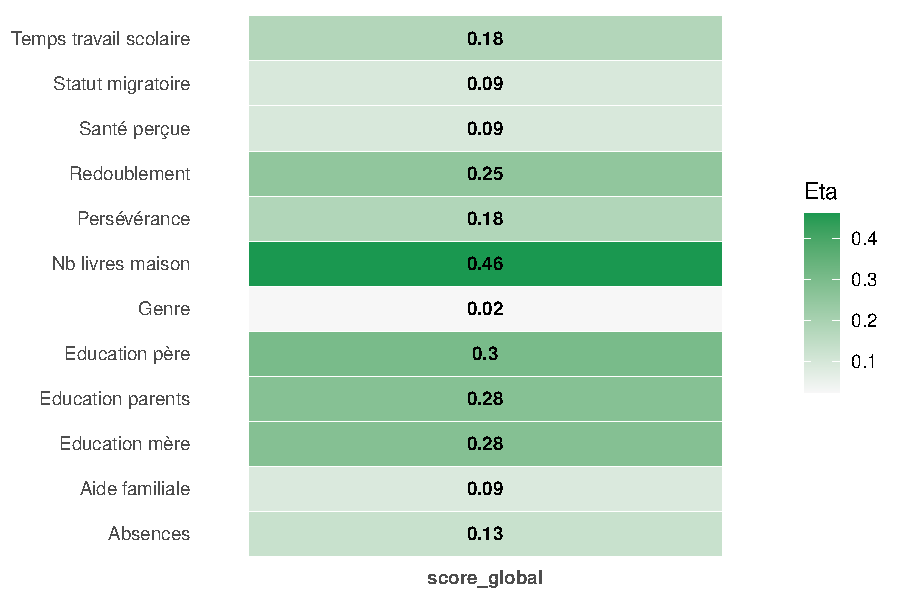
\includegraphics[keepaspectratio]{rapport_files/figure-pdf/fig-10-1.pdf}}

}

\caption{\label{fig-10}}

\end{figure}%

\begin{figure}

\centering{

\begin{table}
\caption*{
{\fontsize{14}{17}\selectfont  \textbf{Top 5 des variables les plus associées au score scolaire global}\fontsize{10}{12}\selectfont } \\ 
{\fontsize{9}{11}\selectfont  PISA 2022 — Pays membres de l’OCDE\fontsize{10}{12}\selectfont }
} 
\fontsize{10.0pt}{12.0pt}\selectfont
\begin{tabular*}{\linewidth}{@{\extracolsep{\fill}}lrl}
\toprule
Variable & Coefficient & Type de lien \\ 
\midrule\addlinespace[2.5pt]
Type de filière & {\cellcolor[HTML]{1A9850}{\textcolor[HTML]{FFFFFF}{0.49}}} & Coefficient η (eta) \\ 
Nombre de livres & {\cellcolor[HTML]{59AD72}{\textcolor[HTML]{FFFFFF}{0.46}}} & Coefficient η (eta) \\ 
Biens matériels & {\cellcolor[HTML]{A3CFAD}{\textcolor[HTML]{000000}{0.41}}} & Corrélation de Pearson (r) \\ 
Statut socio-économique & {\cellcolor[HTML]{A3CFAD}{\textcolor[HTML]{000000}{0.41}}} & Corrélation de Pearson (r) \\ 
Statut professionnel parental & {\cellcolor[HTML]{F7F7F7}{\textcolor[HTML]{000000}{0.35}}} & Corrélation de Pearson (r) \\ 
\bottomrule
\end{tabular*}
\begin{minipage}{\linewidth}
\vspace{.05em}
\textbf{Lecture :} plus le coefficient est proche de 1, plus le lien avec le score scolaire global est fort.\\
\end{minipage}
\end{table}

}

\caption{\label{fig-11}Tableau des 5 vairables les plus liées au score
global}

\end{figure}%

Intuitivement, on pourrait penser que la quantité et la qualité des
ressources éducatives à disposition des élèves en dehors du temps
scolaire sont liées à leur réussite scolaire. Or, nous avons déja
étudier cette possibilité lors de l'étude des variables économiques et
n'en avons pas conclut de lien significatif. Au delà de l'aspect
économique, les ressources mise à disposition de l'enfant représentent
également les choix d'investissement des parents quant à la scolarité de
leurs enfants.Il nous semblait alors important d'évoquer ce point ici.
Ainsi, le niveau de ressources matérielles et culturelles dont dispose
un élève dans son environnement familial n'est pas forcément lié à sa
réussite scolaire. Le niveau global de ressources n'est pas non plus lié
au niveau d'un élève à l'échelle globale, mais cela n'écarte pas le fait
qu'il peut être important dans certaines zones géographiques, ni que
certains types de ressources ne peuvent pas être lié à la réussite
scolaire d'un élève. Concentrons nous sur l'indice du nombre de livres
présent dans le foyer de l'élève. C'est notamment ce qu'on avait montré
à travers la possesion de livre corrélé à la réussite scolaire. On
observe que, que plus un élève à de livre chez lui, plus il réussit à
l'école. Cette corrélation est légèrement plus importante quant à la
réussite en maths, ce qui semble étonnant, puisque la présence devrait
avant tout être associé à une progression en lecture, mais on ne peut
pas exclure que la présence de livre peut inclure des manuels scolaires.
Or la possession de livre semble davantage être le reflet d'une certaine
aisance économique, plus que d'une volonté de transmission à l'enfant.

Au-delà de l'accès à différentes ressources, la réussite scolaire
pourrait être expliquée par l'investissement d'un élève dans ses
devoirs. Sans autres ressources que celles offertes par le système
éducatif, davantage de travail pourrait permettre à l'élève de
progresser. C'est effectivement ce qui ressort de la base de données,
même si la corrélation reste faible. Ainsi la présence de livres au
domicile familial semble davantage significative dans la réussite d'un
élève que son investissement personnel. Nous pourrions voir ici une
forme de déterminisme, au sens où le nombre de livres dont il dispose
dépend davantage de son environnement familial que de caractéristiques
individuelles comme ses efforts personnels.

Nous allons désormais nous concentrer sur l'impact des caractéristiques
parentales sur la réussite de l'enfant à l'école. Tant par leur
parcours, que par leurs actions quotidiennes, les parents jouent un rôle
important dans la construction d'un enfant. C'est ce qu'on appelle la
socialisation primaire. Ainsi il semble intéressant d'étudier leur
impact sur la réussite scolaire. Dans un optique de reproduction
sociale, nous pouvons nous demander si le niveau d'éducation est lié à
celui des enfants. On remarque que globalement, le niveau d'étude des
parents est corrélé positivement avec la réussite scolaire. On remarque
également que la corrélation avec le niveau d'étude du père est
légèrement plus forte que celle avec celui de la mère. C'est la moyenne
en mathématiques qui semble le plus dépendante du niveau d'étude des
parents.

Cependant, l'aide familiale après l'école, ne permet que peu aux élèves
de réussir puisque même si elle est corrélée positivement au résultats
scolaires, cette corrélation reste négligeable. D'autre part, une
observation étonnante est issue de la base de donnée. L'implication
parentale ( la valorisation de l'éducation, l'implication dans les
activités scolaires et extra-scolaires ..) est corrélé négativement avec
la moyenne des élèves. Cela suggère que plus un élève a des bonnes
notes, moins ses parents sont impliqués, alors qu'on pourrait penser que
le soutien et l'accompagnement parental jouent un rôle primordial dans
la réussite scolaire. On pourrait interpréter ce résultat de la manière
suivante. Des parents voyant que leur enfant réussi, pourrait lui
laisser davantage d'autonomie quant à l'accompagnement scolaire.

Enfin, nous nous intéressons aux caractéristiques individuelles de
l'élève. On s'intéresse dans un premier temps à l'impact du genre sur la
réussire des élève. D'après le graphique ci-dessous, c'est en science
que les résultats semblent le plus similaires. Cependant, les filles
réussissent mieux que les garçons en lecture et moins bien en qu'eux en
maths.

\begin{figure}

\centering{

\pandocbounded{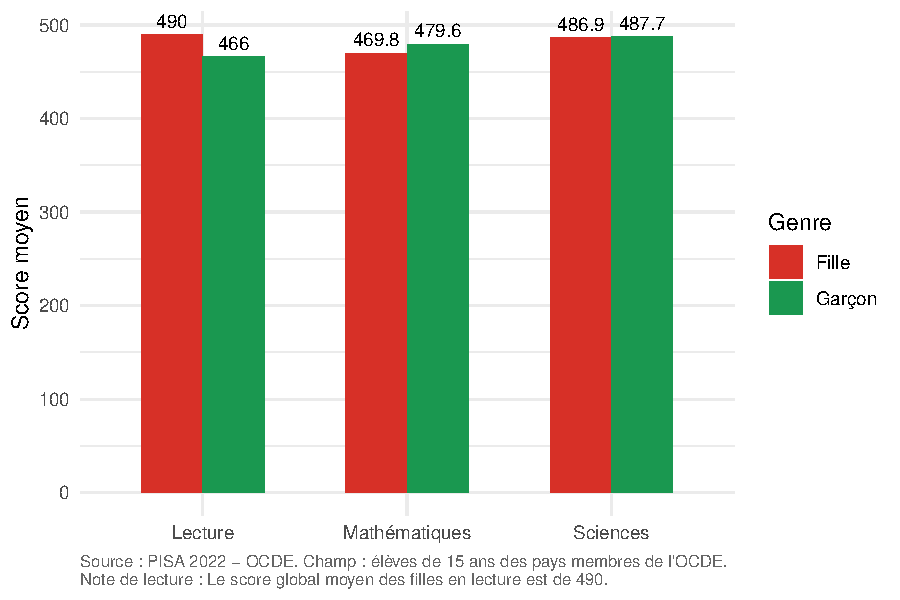
\includegraphics[keepaspectratio]{rapport_files/figure-pdf/fig-12-1.pdf}}

}

\caption{\label{fig-12}Score moyen par matière selon le genre}

\end{figure}%

La persévérance face aux tâches est corrélée positivement à la réussite
scolaire, cependant encore une fois cette corrélation est négligeable.
Il est donc impossible d'observer un lien fort. On pourrait penser que
persévérer fait progresser, mais des élèves en difficulté pourraient
avoir besoin d'effectuer un effort extrêmement important pour peu de
résultat. Il est aussi important à prendre en compte que plus de la
moitié des interrogés n'ont pas répondu, ce résultat est donc biaisé. De
la même manière l'état de santé des élèves est corrélée positivement
avec la réussite scolaire, cependant cette corrélation reste trop faible
pour en tirer une véritable conclusion, d'autant plus que cette variable
présente près de 80\% de non réponse. Ainsi, il est possible que si
100\% des intérrogés avaient répondu, les résultats auraient été
complétement différent. Même si il semble au premier abord évident qu'un
élève en bonne santé, dispose de meilleures conditions pour performer à
l'école.

On s'intéresse désormais à l'impact des migrations sur la réussite
scolaire. On rappelle la signification des issues: 1 : élève né dans le
pays dont les parents sont nés dans le pays, 2: élève né dans le pays
dont au moins un parent est né à l'étranger, 3: élève né à l'étranger.
On remarque avec les graphiques suivants que les élèves de la catégorie
1 réussissent mieux que ceux de la catégorie 2 qui réussissent mieux que
ceux de la catégorie 3. Cela pourrait être lié à la barrière de la
langue. Un enfant ne parlant pas couramment la langue parlé à l'école
rencontrera davantage de difficultés dans son apprentissage.

\begin{figure}

\centering{

\pandocbounded{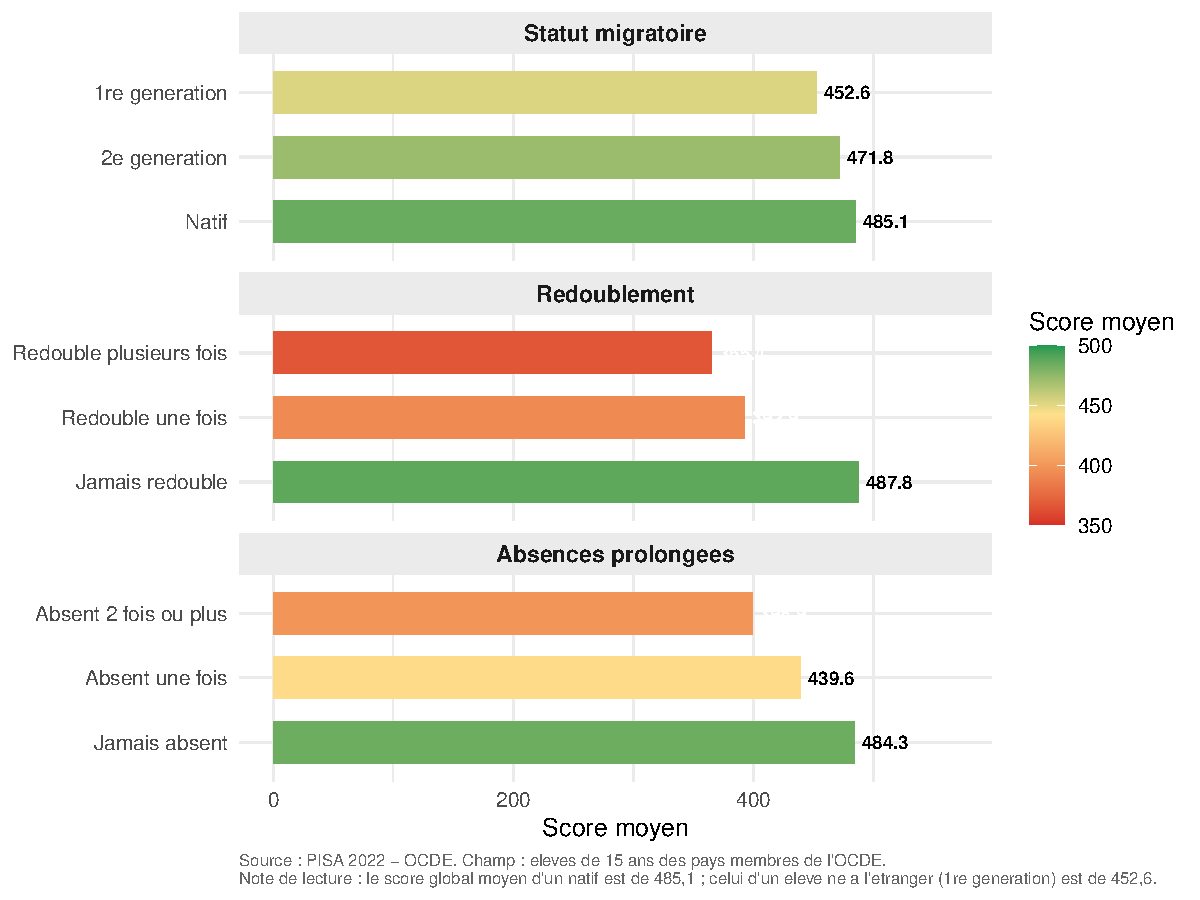
\includegraphics[keepaspectratio]{rapport_files/figure-pdf/fig-13-1.pdf}}

}

\caption{\label{fig-13}Score moyen selon le parcours individuel de
l'élève}

\end{figure}%

On s'intéresse désormais au lien entre redoublement et réussite
scolaire. Ce lien peut être double, un élève qui redouble est en
difficulté, mais l'objectif du redoublement et de lui permettre de
réussir. Il est aussi important de noter que certains pays de l'OCDE ne
pratiquent pas ou très peu le redoublement. On remarque que les élèves
n'ayant jamais redoublé ont en moyenne de meilleures moyennes que ceux
qui ont redoublé une fois qui ont eu des meilleures moyennes que ceux
qui ont redoublé plusieurs fois. C'est le cas tant en science, qu'en
mathématiques et qu'en lecture.

Pour finir, nous nous intéressons à l'impact des absences prolongées sur
la réussite scolaire. La valeur 1 signifie que l'élève n'a jamais eu
d'absence prolongée, la valeur 2 que c'est arrivé une fois et la valeur
3 que c'est arrivé 2 fois ou plus. La question prend en compte les
années de l'ISCED 1, 2 et 3 c'est -à -dire du primaire au lycée. Encore
une fois les élèves n'ayant jamais eu d'absence prolongé réussissent
mieux que ceux qui en ont eu une qui réussissent mieux que ceux qui en
ont eu 2 ou plus. Cependant, cette conclusion reste à nuancer, puisque
cette analyse est basé sur seulement trois quarts des sondés compte
tenue des non-réponses.

Finalement, l'ensemble des ressources que possède l'élève n'est pas lié
à sa réussite, même si la possession de certaines ressources
particulières peut l'être. Son investissement personnel ne l'est pas non
plus. L'influence parentale est elle aussi partagé quant à la réussite
scolaire. Le niveau socio-professionel joue un rôle mais l'implication
de ces derniers est faiblement corrélés négativement au niveau scolaire
de l'enfant. Enfin, le genre, la persévérance et la santé de l'élève
sont faiblement liés à sa réussite sans pour autant que lien
significatif émerge. L'immigration, le redoublement et les absences
prolongées sont également faiblement lié à la réussite de l'élève.

Ainsi, à l'échelle individuelle, certaines variables influencent les
résultats scolaires et sont donc à l'origine d'inégalité. Le patrimoine
économique et culturel d'un individu joue un rôle, plus il évolue dans
un environnement aisé, meilleur sont ses notes. Dans le domaine
scolaire, l'influence de l'établissement fréquenté reste faible et le
nombre d'heure de mathématiques hebdomadaire et même indépendant du
niveau scolaire. C'est davantage le parcours individuel via les
redoublements mais surtout le type de filière suivi qui affecte
réellement la réussite d'un élève. Dans le domaine socio-familial, seul
le niveau socio-professionnel des parents influence significativement la
réussite scolaire. D'autres variables l'influencent mais pas de manière
significative.

\chapter{II --- Les vecteurs d'inégalités scolaires sont-ils les mêmes
au sein de tous les pays de
l'OCDE}\label{ii-les-vecteurs-dinuxe9galituxe9s-scolaires-sont-ils-les-muxeames-au-sein-de-tous-les-pays-de-locde}

Nous avons identifié à l'échelle individuelle les variables qui affecte
la trajectoire scolaire d'un élève étudiant dans un pays de l'OCDE.
Désormais, nous allons changer d'échelle.Nous souhaitons vérifier si à
l'échelle nationale ce sont les mêmes caractéristiques qui définissent
le niveau scolaire d'un pays sur la scène internationale. Ainsi nous
avons regrouper les pays en trois catégories : fort, moyen et faible
selon les résultats des élèves qui y étudient.

\begingroup\fontsize{8}{10}\selectfont

\begin{longtable}[t]{lrrrrrrrrrr}
\caption{\label{tab:unnamed-chunk-2}Moyennes des variables par groupe de pays}\\
\toprule
groupe & ESCS & SCHSUST & PQSCHOOL & ST059Q01TA & ST059Q02JA & EXPO21ST & HISEI & HOMEPOS & LEARRES & PARINVOL\\
\midrule
\cellcolor[HTML]{f8d7da}{En difficulté} & \cellcolor[HTML]{f8d7da}{-0.22} & \cellcolor[HTML]{f8d7da}{-0.07} & \cellcolor[HTML]{f8d7da}{0.21} & \cellcolor[HTML]{f8d7da}{4.97} & \cellcolor[HTML]{f8d7da}{27.82} & \cellcolor[HTML]{f8d7da}{0.03} & \cellcolor[HTML]{f8d7da}{50.80} & \cellcolor[HTML]{f8d7da}{-0.34} & \cellcolor[HTML]{f8d7da}{0.10} & \cellcolor[HTML]{f8d7da}{0.25}\\
\cellcolor[HTML]{fff3cd}{Résultats intermédiaires} & \cellcolor[HTML]{fff3cd}{0.05} & \cellcolor[HTML]{fff3cd}{0.12} & \cellcolor[HTML]{fff3cd}{-0.12} & \cellcolor[HTML]{fff3cd}{4.29} & \cellcolor[HTML]{fff3cd}{27.75} & \cellcolor[HTML]{fff3cd}{-0.03} & \cellcolor[HTML]{fff3cd}{53.02} & \cellcolor[HTML]{fff3cd}{0.12} & \cellcolor[HTML]{fff3cd}{0.08} & \cellcolor[HTML]{fff3cd}{0.05}\\
\cellcolor[HTML]{d4edda}{Meilleurs résultats} & \cellcolor[HTML]{d4edda}{0.19} & \cellcolor[HTML]{d4edda}{0.00} & \cellcolor[HTML]{d4edda}{-0.18} & \cellcolor[HTML]{d4edda}{4.35} & \cellcolor[HTML]{d4edda}{26.23} & \cellcolor[HTML]{d4edda}{0.02} & \cellcolor[HTML]{d4edda}{56.33} & \cellcolor[HTML]{d4edda}{0.24} & \cellcolor[HTML]{d4edda}{-0.15} & \cellcolor[HTML]{d4edda}{-0.27}\\
\bottomrule
\multicolumn{11}{l}{\rule{0pt}{1em}NOTE DE LECTURE : Dans les pays en difficulté, la valeur de l'indice ESCS est en moyenne de -0,22.}\\
\end{longtable}
\endgroup{}

\section{A --- Le capital économique affecte-t-il la réussite scolaire
uniformément au sein de
l'OCDE}\label{a-le-capital-uxe9conomique-affecte-t-il-la-ruxe9ussite-scolaire-uniformuxe9ment-au-sein-de-locde}

Nous avons vu dans la première partie qu'à l'échelle individuelle
certaines variables économiques étaient liées à la réussite scolaire
d'un élève. Nous voulons maintenant savoir si ces mêmes variables
influencent le niveau scolaire d'un pays par rapport aux autres dans
l'OCDE. Ainsi, nous avons calculer la moyenne pour chaque groupe de pays
des variables significatives à l'échelle individuelles.

\begin{figure}

\centering{

\begingroup\fontsize{8}{10}\selectfont

\begin{longtable*}[t]{lrrrrrrrrrr}
\toprule
groupe & ESCS & SCHSUST & PQSCHOOL & ST059Q01TA & ST059Q02JA & EXPO21ST & HISEI & HOMEPOS & LEARRES & PARINVOL\\
\midrule
\cellcolor[HTML]{f8d7da}{En difficulté} & \cellcolor[HTML]{f8d7da}{-0.22} & \cellcolor[HTML]{f8d7da}{-0.07} & \cellcolor[HTML]{f8d7da}{0.21} & \cellcolor[HTML]{f8d7da}{4.97} & \cellcolor[HTML]{f8d7da}{27.82} & \cellcolor[HTML]{f8d7da}{0.03} & \cellcolor[HTML]{f8d7da}{50.80} & \cellcolor[HTML]{f8d7da}{-0.34} & \cellcolor[HTML]{f8d7da}{0.10} & \cellcolor[HTML]{f8d7da}{0.25}\\
\cellcolor[HTML]{fff3cd}{Résultats intermédiaires} & \cellcolor[HTML]{fff3cd}{0.05} & \cellcolor[HTML]{fff3cd}{0.12} & \cellcolor[HTML]{fff3cd}{-0.12} & \cellcolor[HTML]{fff3cd}{4.29} & \cellcolor[HTML]{fff3cd}{27.75} & \cellcolor[HTML]{fff3cd}{-0.03} & \cellcolor[HTML]{fff3cd}{53.02} & \cellcolor[HTML]{fff3cd}{0.12} & \cellcolor[HTML]{fff3cd}{0.08} & \cellcolor[HTML]{fff3cd}{0.05}\\
\cellcolor[HTML]{d4edda}{Meilleurs résultats} & \cellcolor[HTML]{d4edda}{0.19} & \cellcolor[HTML]{d4edda}{0.00} & \cellcolor[HTML]{d4edda}{-0.18} & \cellcolor[HTML]{d4edda}{4.35} & \cellcolor[HTML]{d4edda}{26.23} & \cellcolor[HTML]{d4edda}{0.02} & \cellcolor[HTML]{d4edda}{56.33} & \cellcolor[HTML]{d4edda}{0.24} & \cellcolor[HTML]{d4edda}{-0.15} & \cellcolor[HTML]{d4edda}{-0.27}\\
\bottomrule
\end{longtable*}
\endgroup{}

}

\caption{\label{fig-15}moyennes des variables par groupe par pays}

\end{figure}%

Afin de rendre l'analyse du tableau ci dessus plus claire, il est
important de rappeler que ESCS est composé d'HOMEPOS et que ces deux
variables ainsi que LEARRES sont des variables standardisées. L'indice
ESCS est à l'échelle individuelle fortement lié au niveau scolaire. Il
est important de prendre des pincettes lors de l'analyse à l'échelle
macroéconomque puisqu'on efface les inégalités au sein d'un même pays.
On constate à cette échelle qu'une relation existe bel et bien. Il
existe un écart de 0,48 point entre le groupe faible et le groupe fort,
ce qui reste modeste pour un indice standardisé. On constate également
une asymétrie. L'écart entre le groupe faible et moyen est prés de 4
fois supérieur à celui entre le groupe moyen et fort. On peut en
conclure que le statut socio-économique joue surtout par le bas. Un
faible niveau ESCS semble davantage pénalisant qu'un indice élevé est
bénéfique. Ainsi, la pauvreté des milieux scolaires serait un frein plus
puissant que la richesse n'en serait un accélérateur. On pourrait aussi
imaginer un effet de seuil. Au-delà d'un certain niveau
socio-économique, l'ESCS cesse d'être le facteur déterminant du niveau
scolaire d'un pays.

Du fait de la composition de l'indice, on observe une tendance similaire
pour les possesions matérielles, avec un effet légèrement plus amplifié.

De plus, à l'échelle individuelle la possession de livres est lié au
niveau scolaire. On retrouve également cette intuition à l'échelle
nationale. Comme l'indice ESCS l'écart est plus important entre les pays
faibles et moyens qu'entre le groupe moyen et fort. Cependant les écarts
ne sont pas comparables entre les deux indices.L'indice ESCS est un
indice standardisé alors que ST255Q01JA est une variable ordinale codée
numérique. Si on se rapporte au code de l'indice, l'entier dont sont le
plus proche trois moyennes est 4. Cela correspont à la présence de 26 à
100 livres au domicile familial. De cette manière, l'écart ne semble
plus aussi significatif.

Quant à l'indice LEARRES, il peut être à la fois interpréter comme
résultant de l'environnement scolaire et des ressources que l'école met
à disposition de l'élève en dehors du temps scolaire que comme
représentatif du niveau économique du ménage. A l'échelle individuelle,
on constatait une absence totale de corrélation avec le niveau scolaire.
Cependant à l'échelle nationale, le résultat est autre et peut être
contre intuitif. Une valeur élevé de cet indice signfie que lors des
fermetures d'école l'élève à eu accès a davantage de ressources variées
qu'une valeur faible. Une valeur faible peut ainsi traduire à la fois un
manque d''équipement ou un manque de suivi de la part de l'école. On
constate à l'échelle nationale que dans le groupe faible les élèves ont
eu accès à davantage de ressources que dans les pays forts et moyens
dont la moyenne est similaire à 0,02 point de pourcentage près. Ce
résultat interpèle puisque le niveau de capital socio-économique est lié
au niveau scolaire. On pourrait penser que autant les pays avec un
indice ESCS élevé que ses habitants disposent de davantage de moyens
pour permettre le suivi de l'école à distance et qu'ainsi, l'indice
LEARRES serait plus élevé pour les pays forts or c'est le contraire.
Cela peut s'expliquer par le fait que les pays du groupe faible ont pu
être moins touché par les fermetures d'école ou encore que l'indice
LEARRES mesure la quantité des ressources pédagogiques à dispositif et
non pas la qualité. Enfin, il es possible que les réponses des élèves
soient biaisés. Les élèves des pays faibles pourraient avoir surestimés
leurs ressources disponibles puisqu'ils répondant par rapport à ce qu'il
connaissent.

\section{B --- L'environnement scolaire national est il vecteur des
réussites
?}\label{b-lenvironnement-scolaire-national-est-il-vecteur-des-ruxe9ussites}

Dans la première Partie, nous avons vu que certaines variables liées à
l'environnement scolaire de l'élève avaient en effet un impact sur la
qualité de ses notes. Pour constater cela au niveau des pays, nous avons
décidé de nous pencher à nouveau sur les pays forts et les pays faibles,
mais en nous penchant maintenant sur la différence entre certains
indicateurs pour les 2 types de pays.

\begin{figure}

\centering{

\pandocbounded{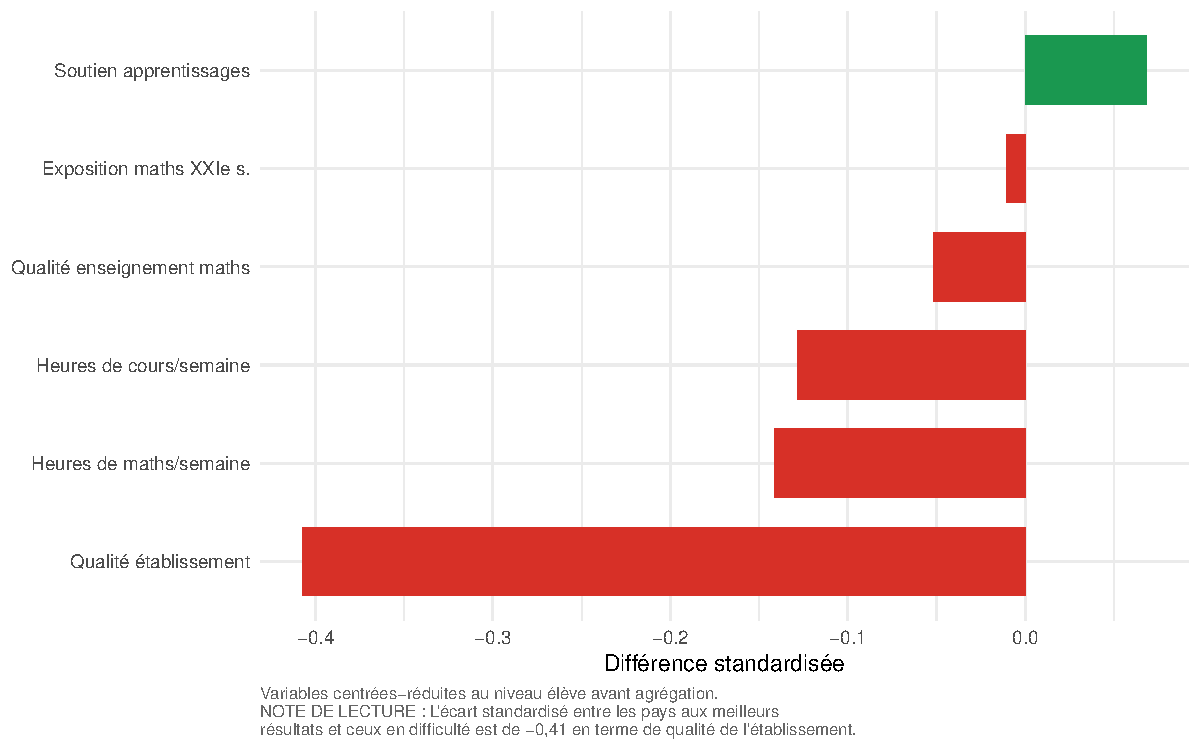
\includegraphics[keepaspectratio]{rapport_files/figure-pdf/fig-17-1.pdf}}

}

\caption{\label{fig-17}écart standardisée entre forts et faibles}

\end{figure}%

On constate sur ce graphique que les résultats sont contre-intuitifs. En
effet, la qualité de l'établissement semble avoir un gros effet négatif
sur la réussite d'un pays, ainsi que le nombre d'heures de cours par
semaine. Le premier point est compliqué à expliquer : Ce dernier point
peut peut être s'expliquer par le fait que les pays de l'OCDE sont
globalement des pays dévellopés avec un nombre décent d'heures de cours
par semaine. Ainsi, il serait faux de dire que moins il y a d'heure de
cours, meilleurs sont les résultats. En effet, il est fort probable
qu'un pays hors OCDE avec très peu d'heures de cours par semaine ait de
bien moins bon résultats qu'un pays de l'OCDE. Seulement, cette
différence s'explique peut être par le fait que les élèves sont plus
épanouis avec moins d'heures de cours, et ont donc de meilleurs
résultats. On peut par exemple prendre le cas de l'Allemagne, qui n'a le
cours que le matin et laisse l'après-midi libre pour des activités
sportives par exemple. Moins d'heure de cours peut aussi dire plus de
travail personnel, ce qui expliquerait aussi les meilleurs résultats.
Enfin, le soutien de l'aprentissage semble être une caractéristique des
pays forts, en effet accompagner tout type d'élèves ne peut que être
bénéfique sur la réussite globale du pays.

Afin d'approfondir le lien entre pays et résultats, nous pouvons aussi
étudier le nuage de points suivant :

\begin{figure}

\centering{

\pandocbounded{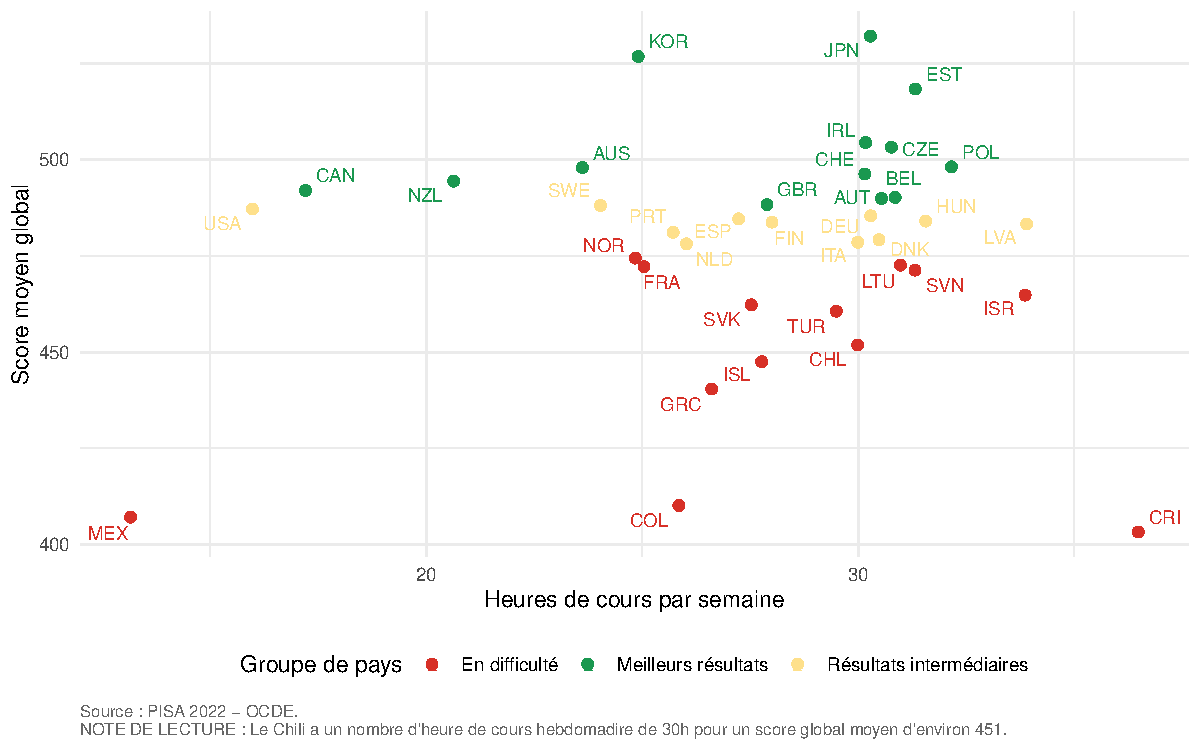
\includegraphics[keepaspectratio]{rapport_files/figure-pdf/fig-18-1.pdf}}

}

\caption{\label{fig-18}Lien entre niveau scolaire moyen et nombre
d'heures de cours}

\end{figure}%

On peut voir ici que à part le Mexique, tout les pays faibles ont un
nombre élevé d'heures de cours par semaine, tandis que dans les pays
forts, il y a des pays tels que le Canada, la Nouvelle-Zelande ou
l'Australie avec un volume horaire faible. Ainsi, ce nuage de points
nous montre que l'augmentation du temps de travail et les résultats
n'ont pas une relation linéaire, et même l'inverse (Le Costa Rica ne
réussit pas bien malgré un très gros volume horaire, tandis que à part
le Mexique, les pays avec un faible volume horaire résusissent bien). Ce
n'est pas non plus décoréllé, car des pays comme la Pologne ou l'Estonie
ont un nombre important d'heures par semaine, et sont quand même dans
les pays forts.

Ainsi, à l'échelle des pays, les variables de l'environnement scolaire
ne présentent pas de lien clair avec la réussite moyenne. En
particulier, le volume horaire ne semble pas déterminant, comme le
montre l'absence de relation linéaire dans le nuage de points. Ces
résultats, parfois contre-intuitifs, suggèrent que la quantité
d'enseignement importe moins que sa qualité. Ils mettent en évidence des
mécanismes différents de ceux observés à l'échelle individuelle.

\section{C- Les caractéristiques socio-familiales et inégalités entre
les
pays}\label{c--les-caractuxe9ristiques-socio-familiales-et-inuxe9galituxe9s-entre-les-pays}

Dans la première partie, nous avons constaté que le niveau d'études des
parents était un facteur très important dans la réussite de l'élève.
Afin d'étudier cette variable au niveau des pays, nous avons pris le
mode de cette variable par pays, c'est à dire la modalité la plus
representé au sein de ce pays.

\begin{figure}

\centering{

\pandocbounded{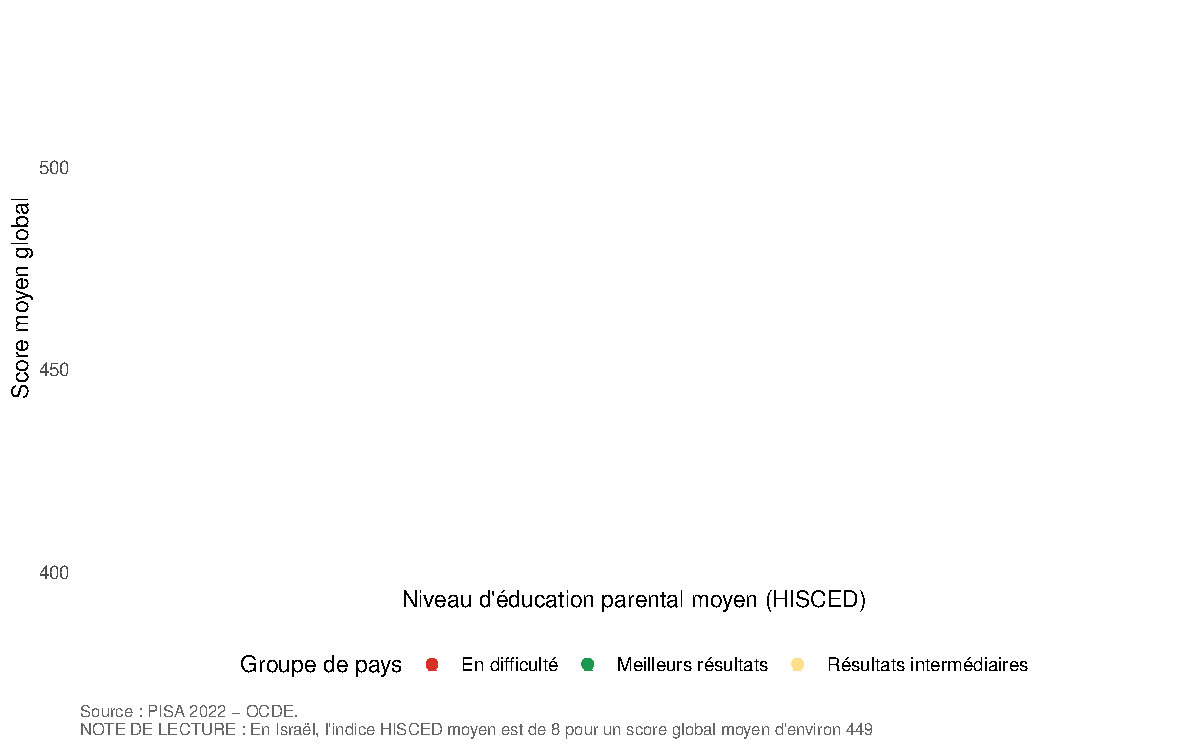
\includegraphics[keepaspectratio]{rapport_files/figure-pdf/fig-19-1.pdf}}

}

\caption{\label{fig-19}Lien entre niveau d'éducation parental (mode) et
performance des pays}

\end{figure}%

Tout d'abord, on constate que touts les pays ont un niveau élevé à
HISCED, le plus bas étant à 3, ce qui correspond à l'équivalent du
baccalauréat. De plus, les pays performants ne sont pas necessairement
ceux avec les niveaux d'études des parents les plus hauts. On peut par
exemple prendre l'exemple de la République Tchèque, l'Autriche ou la
Suisse. Il reste toutetfois compliqué d'analyser ce graphique car la
grande majorité des pays se situent au même niveau (8 et 9), ce qui
laisse peu de dispersion pour étudier les différences.

Désormais, penchons-nous sur les effets de l'immigration. Pour cela,
nous allons nous intéresser à la proportion de migrants de première et
deuxième génération parmis les élèves.

\begin{figure}

\centering{

\pandocbounded{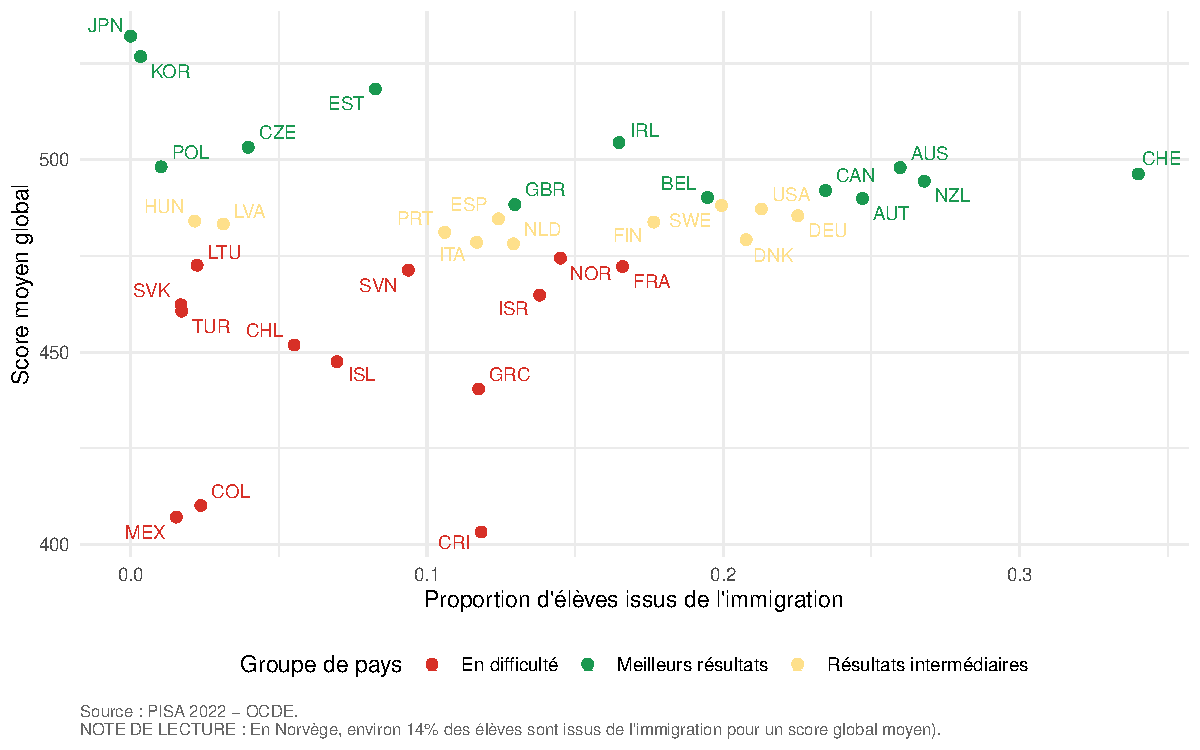
\includegraphics[keepaspectratio]{rapport_files/figure-pdf/fig-20-1.pdf}}

}

\caption{\label{fig-20}Lien entre proportion d'élèves issus de
l'immigration et performance des pays}

\end{figure}%

On constate que la part d'immigrés a très peu d'impact sur les
résultats. Parmis les pays forts, il existe des pays avec très peu et
beuacoup d'immigration (Japon et Suisse par exemple). Parmis les pays
faibles, il y a moins d'immigration, ce qui est lié à l'attractivité
plus faible de ces pays, comme par exemple le Mexique et la Colombie.

Pour les absences, nous allons nous intéresser à la proportion d'élèves
ayant au moins une absence prolongée

\begin{figure}

\centering{

\pandocbounded{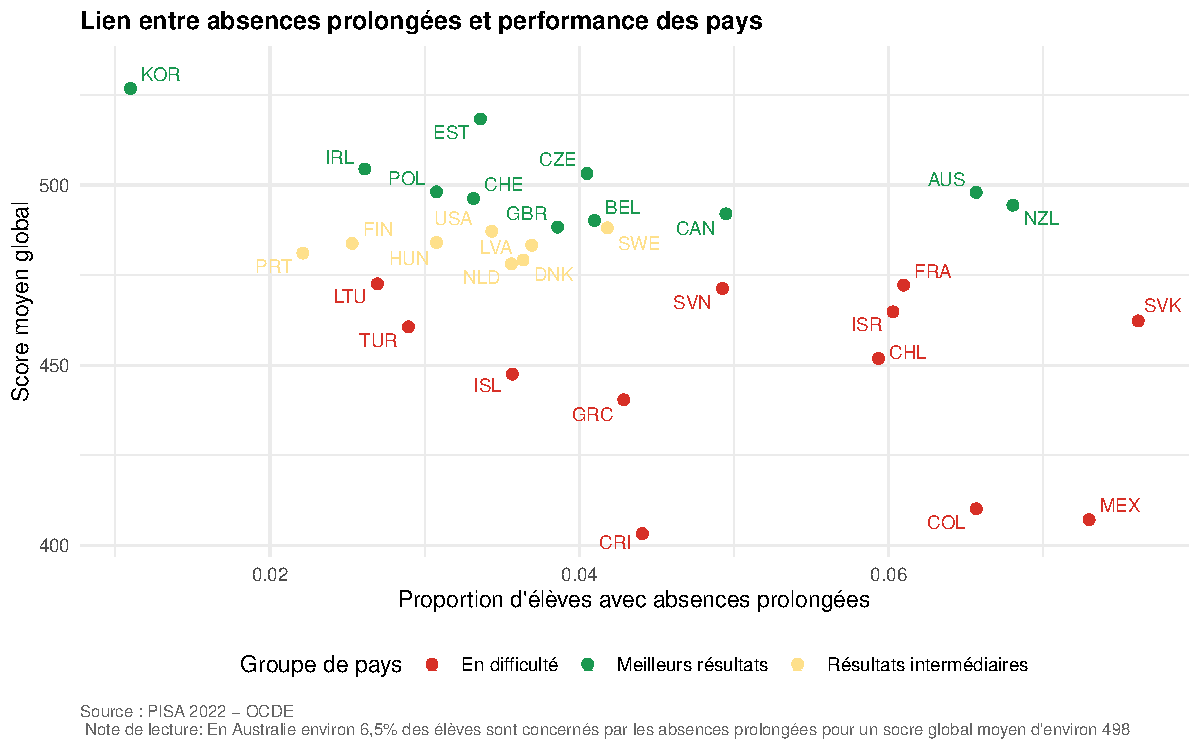
\includegraphics[keepaspectratio]{rapport_files/figure-pdf/fig-21-1.pdf}}

}

\caption{\label{fig-21}lien entre absences prolongées et performance des
pays}

\end{figure}%

Ici, le lien semble être plus clair. En effet, la plupart des pays
faibles ont une proportion plus élevée d'absentéisme, tandis que les
pays les plus performants présentent globalement des taux d'absences
plus faibles. La tendance négative observée suggère que l'assiduité des
élèves joue un rôle important dans la réussite scolaire à l'échelle
nationale. Contrairement à certaines variables étudiées précédemment,
l'absentéisme apparaît donc comme un facteur plus directement associé
aux écarts de performance entre pays, même si quelques exceptions
subsistent.

Ainsi, contrairement aux variables liées à l'environnement scolaire,
certaines caractéristiques socio-familiales apparaissent davantage liées
aux écarts de performance entre pays. Si le niveau d'éducation des
parents est difficile à exploiter ici en raison d'un manque de
dispersion, d'autres facteurs comme l'absentéisme montrent un lien plus
clair avec la réussite scolaire. À l'inverse, la part d'élèves issus de
l'immigration ne semble pas constituer un facteur déterminant à elle
seule. Dans l'ensemble, ces résultats suggèrent que les inégalités entre
pays s'expliquent en partie par des facteurs sociaux et comportementaux,
plus que par les seules caractéristiques du système éducatif.

\chapter{III --- Mise en évidence des facteurs structurants des
inégalités scolaires : une approche par
ACP}\label{iii-mise-en-uxe9vidence-des-facteurs-structurants-des-inuxe9galituxe9s-scolaires-une-approche-par-acp}

\section{A --- Un axe structuré par le capital socio-économique (ESCS,
HISEI,
HOMEPOS)}\label{a-un-axe-structuruxe9-par-le-capital-socio-uxe9conomique-escs-hisei-homepos}

Avant de présenter les résultats, il convient d'expliciter un choix
méthodologique qui conditionne la construction de l'ACP. Parmi les
variables retenues dans les parties précédentes, deux d'entre elles ne
sont pas renseignées pour 28 pays sur les 37 que compte notre
échantillon. Les inclure aurait contraint à n'analyser qu'une poignée de
pays, ce qui aurait rendu l'analyse à la fois statistiquement fragile et
géographiquement peu représentative de l'OCDE. Nous avons donc fait le
choix de les exclure des variables actives, au profit d'un échantillon
de 25 pays.

Les scores scolaires sont quant à eux introduits en variables
supplémentaires : ils ne participent pas à la construction des axes mais
sont projetés a posteriori dans le plan factoriel. Ce choix est
délibéré, il s'agit d'évaluer dans quelle mesure les structures
identifiées à partir des seules variables contextuelles correspondent
aux inégalités de performance scolaire, sans que ces dernières
n'influencent l'analyse.

L'ACP est une méthode de réduction de dimension qui synthétise un
ensemble de variables corrélées en un nombre réduit d'axes orthogonaux,
appelés \textbf{composantes principales}. Chaque axe capture une
fraction de la variance totale du nuage de points. Les variables sont
normalisées avant l'analyse, ce qui garantit que les différences
d'échelle entre indices standardisés et variables brutes n'introduisent
pas de biais dans la construction des axes.

Choix du nombre d'axes retenus

L'éboulis des valeurs propres et le tableau associé permettent de
déterminer le nombre d'axes à retenir. Selon la règle de Kaiser, on
conserve les composantes dont la valeur propre est supérieure à 1 qui
est le seuil en dessous duquel un axe explique moins de variance qu'une
variable originale prise isolément. Trois axes satisfont donc ce
critère. Les deux premiers axes expliquent à eux seuls \textbf{66,4 \%
de la variance totale}, ce qui est un résultat satisfaisant pour une ACP
sur données agrégées par pays. Le troisième axe porte 15,4 \% de
variance supplémentaire, portant le cumul à 81,8 \%. Dans la suite de
l'analyse, nous nous concentrons sur le plan factoriel formé par les
deux premières dimensions, qui constituent la représentation la plus
synthétique et la plus lisible de la structure des pays de l'OCDE.

\begin{figure}

\centering{

\begingroup\fontsize{9}{11}\selectfont

\begin{longtable}[t]{llrrr}
\caption{\label{tab:fig-24}Valeurs propres et variance expliquée (5 premiers axes)}\\
\toprule
 & Axe & Valeur propre & \% variance & \% cumulé\\
\midrule
\textbf{comp 1} & \textbf{Dim.1} & \textbf{3.30} & \textbf{41.20} & \textbf{41.20}\\
\textbf{comp 2} & \textbf{Dim.2} & \textbf{2.02} & \textbf{25.23} & \textbf{66.43}\\
\textbf{comp 3} & \textbf{Dim.3} & \textbf{1.23} & \textbf{15.41} & \textbf{81.83}\\
comp 4 & Dim.4 & 0.78 & 9.80 & 91.63\\
comp 5 & Dim.5 & 0.40 & 4.99 & 96.62\\
\bottomrule
\end{longtable}
\endgroup{}

}

\caption{\label{fig-24}acp-scree}

\end{figure}%

\begin{figure}

\centering{

\pandocbounded{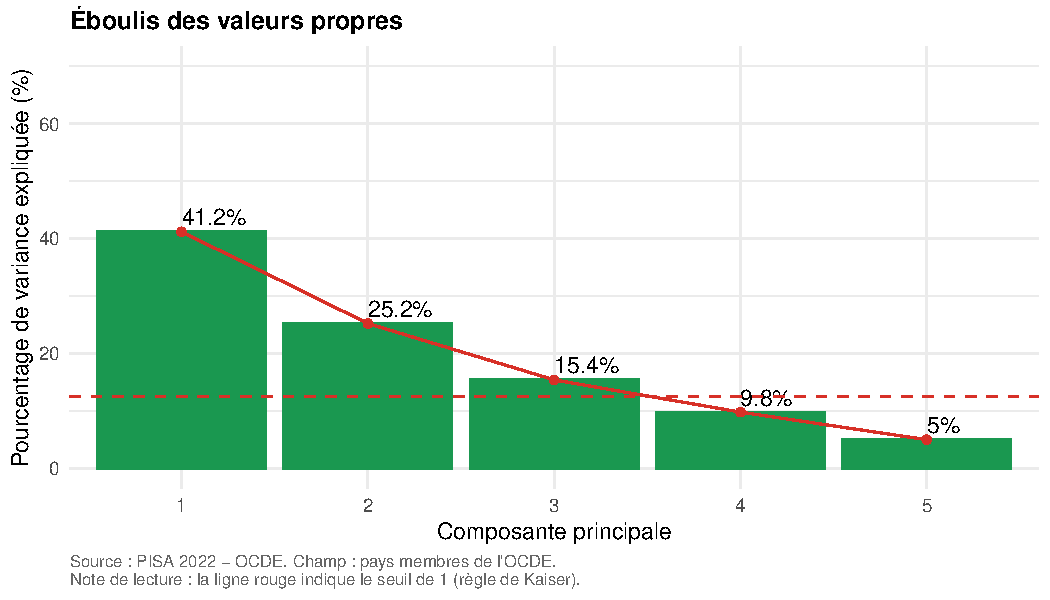
\includegraphics[keepaspectratio]{rapport_files/figure-pdf/fig-25-1.pdf}}

}

\caption{\label{fig-25}-acp-eig-plot}

\end{figure}%

\section{B --- Une opposition entre capital socio-économique et
organisation
scolaire}\label{b-une-opposition-entre-capital-socio-uxe9conomique-et-organisation-scolaire}

Le cercle des corrélations représente les variables actives dans le plan
Dim.1 × Dim.2. La longueur d'une flèche indique la qualité de
représentation de la variable dans ce plan (cos²) : plus elle est proche
du cercle unité, mieux la variable est captée par les deux premiers
axes. L'orientation indique la corrélation avec chaque dimension. Les
variables pointant dans la même direction sont positivement corrélées
entre elles dans cet espace ; des variables à angle droit sont
indépendantes dans ce plan.

\begin{figure}

\centering{

\pandocbounded{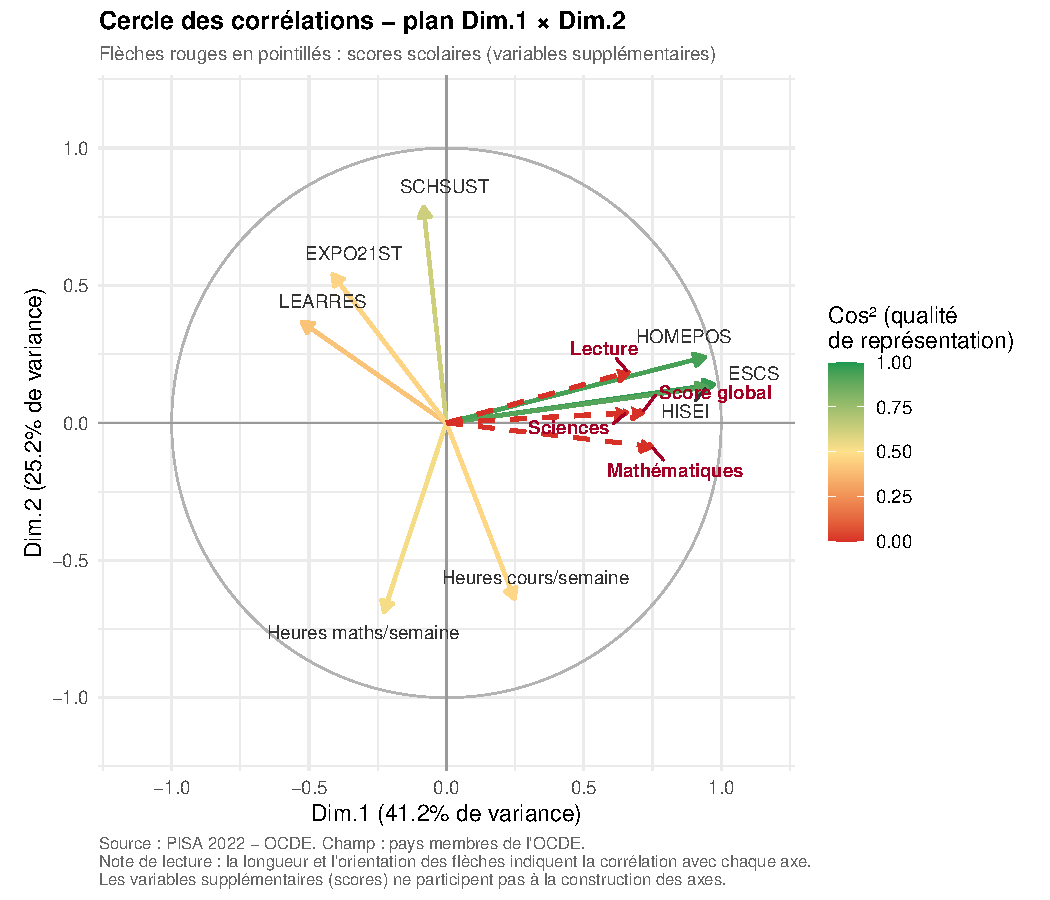
\includegraphics[keepaspectratio]{rapport_files/figure-pdf/fig-26-1.pdf}}

}

\caption{\label{fig-26}-acp-cercle}

\end{figure}%

D'après le graphique de contribution aux axes en annexe, le premier axe
--- qui concentre à lui seul 41 \% de la variance --- structure les pays
selon leur niveau de capital socio-économique. Trois variables
contribuent fortement à cet axe et pointent toutes dans la même
direction : l'indice composite de statut socio-économique et culturel
des familles, le statut professionnel le plus élevé des parents, et la
possession de biens matériels au domicile. Cette convergence traduit
leur forte intercorrélation. Ce qui est cohérent avec le fait que ces
trois dimensions mesurent la richesse familiale. Les scores scolaires,
introduits comme variables supplémentaires, se projettent dans cette
même direction et sont très proches du cercle unité. Cette proximité
suggère une association forte entre le capital socio-économique national
et la performance scolaire, sans qu'on puisse toutefois en conclure un
lien de causalité direct. L'agrégation au niveau national peut masquer
des mécanismes plus complexes à l'œuvre au sein de chaque pays.

À l'opposé sur cet axe, les ressources éducatives mises à disposition
des élèves lors des fermetures d'école pointent dans la direction
inverse. Ce résultat, contre-intuitif au premier abord, avait déjà été
identifié à l'échelle individuelle en partie I : cette variable ne
semble pas fonctionner comme un simple indicateur de richesse ou de
réussite. Il est possible qu'elle capte davantage un contexte sanitaire
particulier, les fermetures liées à la pandémie, qu'un avantage
structurel durable pour les élèves.

Le second axe qui représente \textbf{25 \% de variance} capture une
logique davantage organisationnelle. D'un côté, le nombre d'heures
hebdomadaires de cours et le nombre d'heures de mathématiques par
semaine tirent cet axe vers le bas, caractérisant des systèmes à forte
intensité horaire. De l'autre, le soutien institutionnel de
l'établissement aux apprentissages et l'exposition aux mathématiques
contemporaines tirent dans le sens opposé, caractérisant des systèmes
qui privilégient un accompagnement qualitatif plutôt que quantitatif. Il
serait toutefois hasardeux d'interpréter cette opposition comme un
arbitrage tranché entre quantité et qualité : cet axe traduit avant tout
la diversité des organisations scolaires au sein de l'OCDE, sans qu'on
puisse hiérarchiser ces approches à partir de ce seul plan factoriel.

Un point mérite attention : les scores scolaires sont quasi-orthogonaux
à ce second axe, ce qui signifie que cette dimension organisationnelle
n'est que peu associée aux différences de performance entre pays. Nous
reviendrons sur cette observation dans la partie suivante.

\begin{center}\rule{0.5\linewidth}{0.5pt}\end{center}

\section{C --- Une typologie des pays de l'OCDE selon leur position dans
l'espace
factoriel}\label{c-une-typologie-des-pays-de-locde-selon-leur-position-dans-lespace-factoriel}

La projection des pays dans le plan Dim.1 × Dim.2 permet de visualiser
simultanément leur position relative sur les deux dimensions
identifiées. La taille des points est proportionnelle au score moyen
national, et la couleur correspond au groupe de performance (fort,
moyen, faible) défini en partie II.

\begin{figure}

\centering{

\pandocbounded{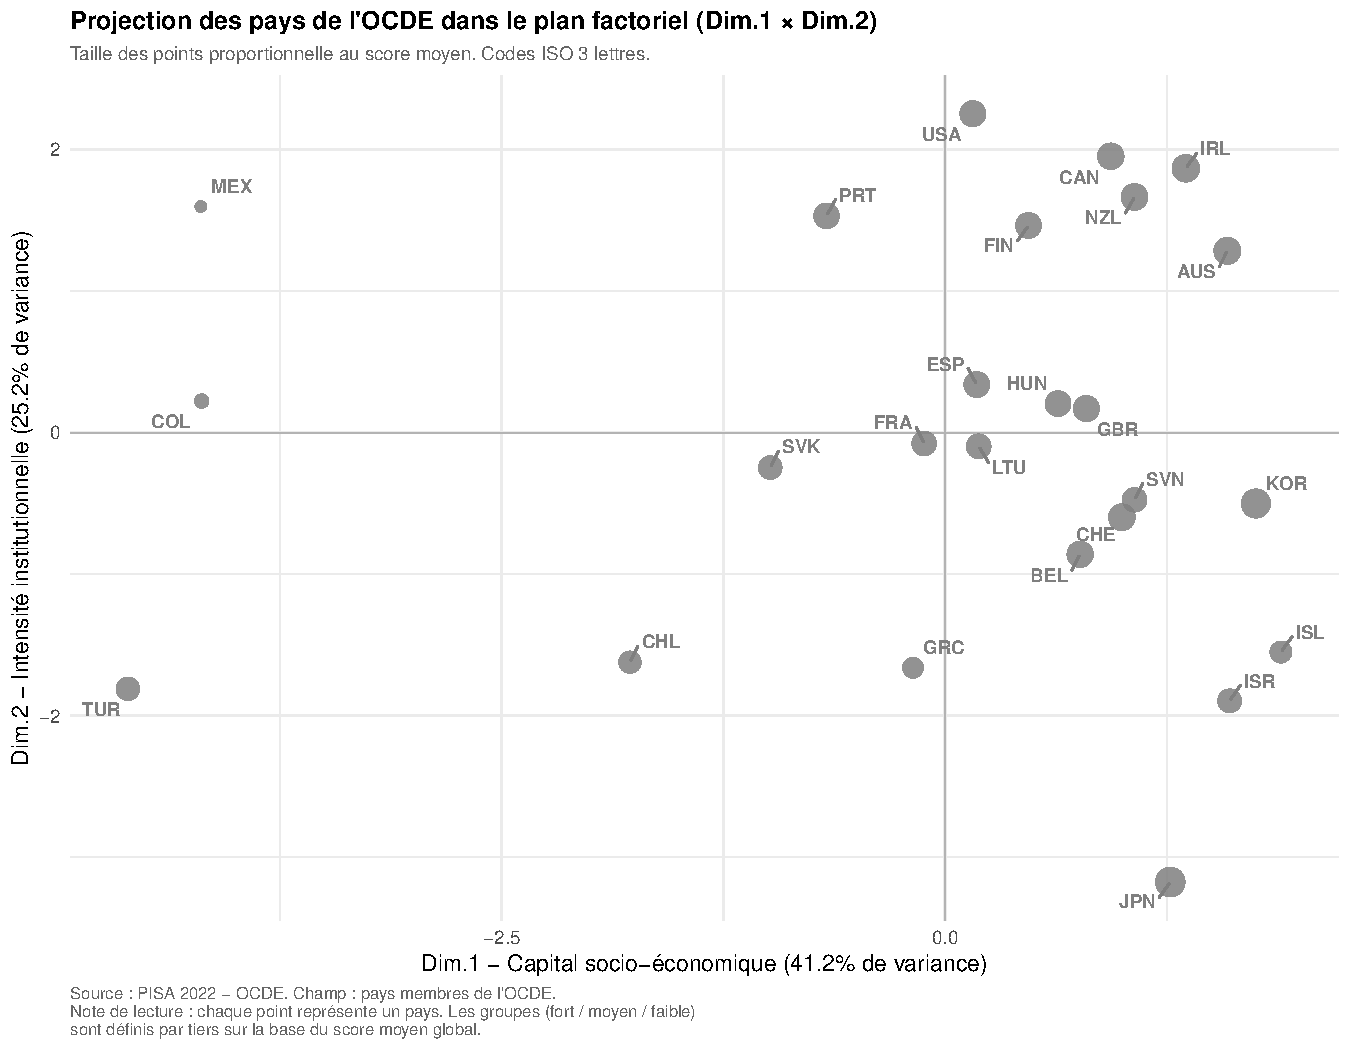
\includegraphics[keepaspectratio]{rapport_files/figure-pdf/fig-27-1.pdf}}

}

\caption{\label{fig-27}-acp-individus}

\end{figure}%

Plusieurs configurations émergent de cette projection :

\textbf{Les pays à fort capital socio-économique et forte performance}
(quadrant droit) regroupent des pays comme la Corée (KOR), la Suisse
(CHE), la Belgique (BEL) ou la Slovénie (SVN). Ils se situent dans les
valeurs positives de Dim.1, confirmant que leur niveau scolaire élevé
s'accompagne d'un contexte socio-économique favorable. Mais Israël (ISR)
et l'Islande (ISL) se trouvent également dans ce quadrant, avec des
performances plus contrastées. Israël étant considéré comme « fort »
malgré une forte dispersion interne, et l'Islance classé dans le groupe
« faible » malgré un ESCS élevé, ce qui en fait un cas atypique sur
lequel nous reviendrons.

\textbf{Les pays à faible capital socio-économique et faible
performance} (quadrant gauche) comprennent le Mexique (MEX), la Colombie
(COL) et le Chili (CHL). Leur position nettement négative sur Dim.1 est
cohérente avec leur classement en bas du tableau des scores. La Turquie
(TUR) occupe une position particulière : très négative sur les deux
axes, elle combine un faible capital socio-économique et une intensité
horaire élevée (valeur basse sur Dim.2), sans que cette dernière ne
semble compenser le premier facteur.

\textbf{Les pays anglophones à organisation scolaire légère} (quadrant
supérieur droit) comme le Canada (CAN), l'Irlande (IRL), l'Australie
(AUS) et la Nouvelle-Zélande (NZL) présentent un capital
socio-économique élevé combiné à des valeurs positives sur Dim.2,
associées à davantage de soutien institutionnel et moins d'heures
formelles. Ce groupe présente des performances solides, ce qui ne permet
pas de conclure que la réduction du volume horaire est préjudiciable à
la réussite.

\textbf{Le Japon (JPN)} occupe une position singulière en bas à droite
du plan : capital socio-économique élevé, mais Dim.2 très négative,
suggérant un système à forte intensité horaire. C'est l'un des pays les
mieux notés de l'OCDE, ce qui illustre qu'un système peut combiner
rigueur institutionnelle et excellence académique.

\textbf{La France (FRA)} se positionne légèrement à droite de l'axe
central (Dim.1 modérément positive) et proche de zéro sur Dim.2, ce qui
la place dans une configuration assez médiane. Son classement au 27e
rang sur 37 suggère que son capital socio-économique moyen, bien que
supérieur à celui des pays les moins favorisés, ne suffit pas à
compenser d'autres facteurs --- notamment une forte dispersion interne
des résultats, qui n'est pas captée par cette ACP réalisée sur des
moyennes nationales.

D'après le graphique de qualité de représentation des pays en annexe,
tous les pays ne sont pas également bien représentés dans le plan Dim.1
× Dim.2. Le cos², compris entre 0 et 1, mesure la part de la variabilité
d'un pays qui est expliquée par les deux premières dimensions. Un cos²
supérieur à 0,7 est généralement considéré comme satisfaisant.

La Turquie, la Colombie, le Mexique et plusieurs autres pays sont très
bien représentés dans ce plan, ce qui signifie que leur positionnement
dans l'OCDE est essentiellement déterminé par les deux grandes
dimensions identifiées.

À l'inverse, des pays comme la France, la Lituanie, la Hongrie ou
l'Espagne présentent des cos² plus faibles, inférieurs à 0,3. Cela
signifie que leur profil est davantage structuré par les axes suivants
(Dim.3 et au-delà), non représentés ici. Ces pays échappent
partiellement à la logique binaire capital socio-économique / intensité
institutionnelle, et mériteraient une analyse complémentaire sur les
dimensions suivantes pour comprendre ce qui les distingue réellement.

Le graphique de synthèse intitulé ``Lien entre l'axe 1 et le score moyen
national'' confronte directement la position de chaque pays sur l'axe 1
de l'ACP à son score moyen national. La corrélation observée est de
\textbf{r = 0,71}, ce qui constitue un résultat notable : le premier axe
de l'ACP étant construit sans aucune information sur les scores
scolaires --- reproduit à lui seul 50 \% de la variance des performances
nationales (r² ≈ 0,50).

Ce résultat vient confirmer, à l'échelle nationale et par une méthode
multivariée, ce que les analyses de corrélation de la partie I avaient
mis en évidence à l'échelle individuelle : le capital socio-économique
des familles est le facteur structural le plus fortement associé aux
inégalités de niveau scolaire au sein de l'OCDE. Ce n'est pas un facteur
parmi d'autres --- c'est la première dimension de différenciation entre
les systèmes éducatifs nationaux.

En revanche, la corrélation entre la deuxième dimension (intensité
institutionnelle) et les scores est quasi nulle (\textbf{r = 0,04}). Ce
résultat invite à la prudence quant aux discours qui font de l'intensité
scolaire un levier principal de la performance nationale. À l'échelle de
l'OCDE, cette dimension distingue certes les pays entre eux, mais elle
ne semble pas structurellement liée à leurs résultats moyens. Cela ne
signifie pas que ces facteurs sont sans effet. Ils peuvent jouer à
d'autres niveaux d'analyse (individuel, local) ou interagir avec
d'autres variables non captées ici mais ils ne constituent pas, à eux
seuls, un déterminant national de la performance scolaire.

Enfin, il convient de rappeler les limites inhérentes à cette ACP.
Travailler sur des moyennes nationales efface la variabilité interne à
chaque pays, qui peut être considérable. Un pays peut afficher un ESCS
moyen élevé tout en présentant de fortes inégalités internes --- or
c'est précisément cette dispersion qui détermine les inégalités
scolaires au sens propre. L'ACP nationale donne une image de la
structure entre pays, non de la structure au sein des pays. Les deux
niveaux d'analyse sont complémentaires et doivent être lus conjointement
pour répondre pleinement à notre problématique.

\chapter{Conclusion}\label{conclusion}

Ce rapport avait pour ambition de comprendre si les sources des
inégalités de niveau scolaire dans les pays de l'OCDE sont les mêmes à
l'échelle individuelle qu'à l'échelle nationale. L'analyse des données
PISA 2022, menée successivement à ces deux niveaux puis confirmée par
une ACP, permet d'apporter des éléments de réponse nuancés à cette
question. À l'échelle individuelle, le capital socio-économique des
familles apparaît comme le facteur le plus structurellement lié à la
réussite scolaire. L'indice ESCS, la possession de biens matériels et le
statut professionnel des parents sont tous positivement corrélés aux
scores des élèves, confirmant l'intuition de nombreux travaux
antérieurs, dont ceux de Bourdieu et Passeron sur la reproduction
sociale. En revanche, certains facteurs que l'on pourrait spontanément
associer à la réussite semblent jouer un rôle bien plus limité
qu'attendu : la présence de ressources éducatives à domicile ou le
nombre d'heures de mathématiques hebdomadaires n'apparaissent pas liés
au niveau scolaire. C'est davantage le type de filière suivi qui semble
constituer le vecteur d'inégalités le plus fort à l'échelle
individuelle, bien qu'il convienne d'interpréter ce résultat avec
prudence, la filière étant souvent le reflet d'orientations précoces
elles-mêmes conditionnées par le milieu socio-économique. À l'échelle
nationale, les résultats convergent en partie avec ce constat, mais
révèlent également des mécanismes propres. Le capital socio-économique
moyen d'un pays reste associé à son niveau de performance, avec
toutefois une asymétrie notable : un faible niveau d'ESCS semble
davantage pénalisant qu'un niveau élevé n'est bénéfique. En revanche,
les variables liées à l'environnement scolaire national produisent des
résultats plus contre-intuitifs. Le volume horaire hebdomadaire, par
exemple, n'entretient pas de relation linéaire claire avec la
performance des pays, ce qui invite à penser que c'est moins la quantité
d'enseignement que sa qualité qui conditionne la réussite à cette
échelle. L'ACP vient confirmer ces résultats : le premier axe factoriel,
structuré autour du capital socio-économique, est corrélé à hauteur de r
= 0,71 avec les scores moyens nationaux, tandis que le second axe,
capturant la diversité des organisations scolaires, n'y est quasiment
pas corrélé (r = 0,04).

En définitive, si le capital socio-économique constitue un facteur
structurant commun aux deux niveaux d'analyse, les variables scolaires
et socio-familiales n'opèrent pas de la même manière selon que l'on
observe un élève ou un pays. Ces résultats appellent néanmoins à la
prudence : les corrélations observées ne permettent pas d'établir des
relations de causalité, et le travail sur des moyennes nationales efface
une variabilité interne qui peut être considérable.

\chapter{Annexe}\label{annexe}

\begin{figure}

\centering{

\pandocbounded{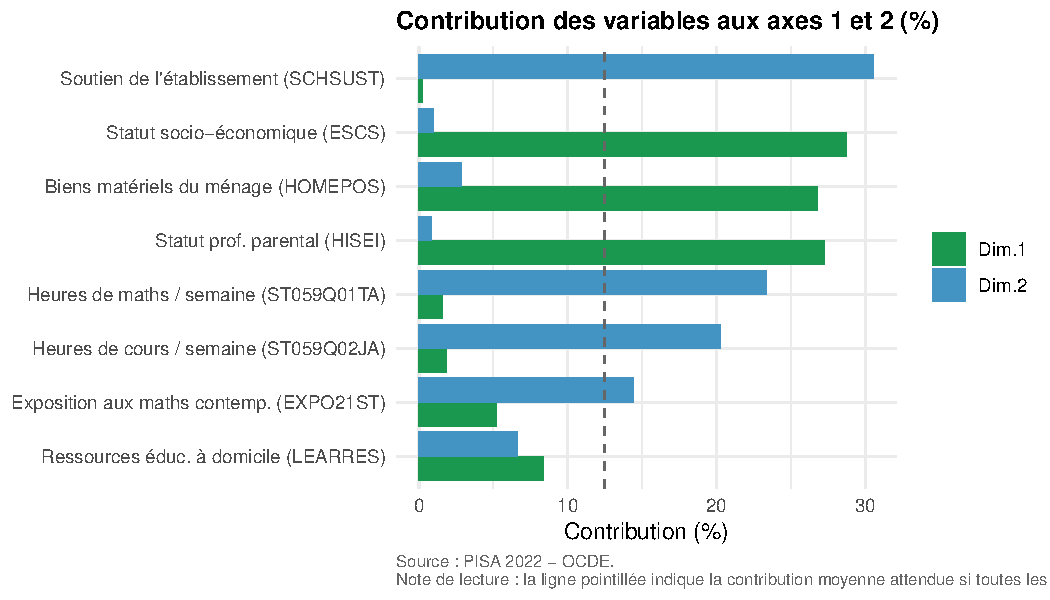
\includegraphics[keepaspectratio]{rapport_files/figure-pdf/fig-28-1.pdf}}

}

\caption{\label{fig-28}-acp-contrib}

\end{figure}%

\begin{figure}

\centering{

\pandocbounded{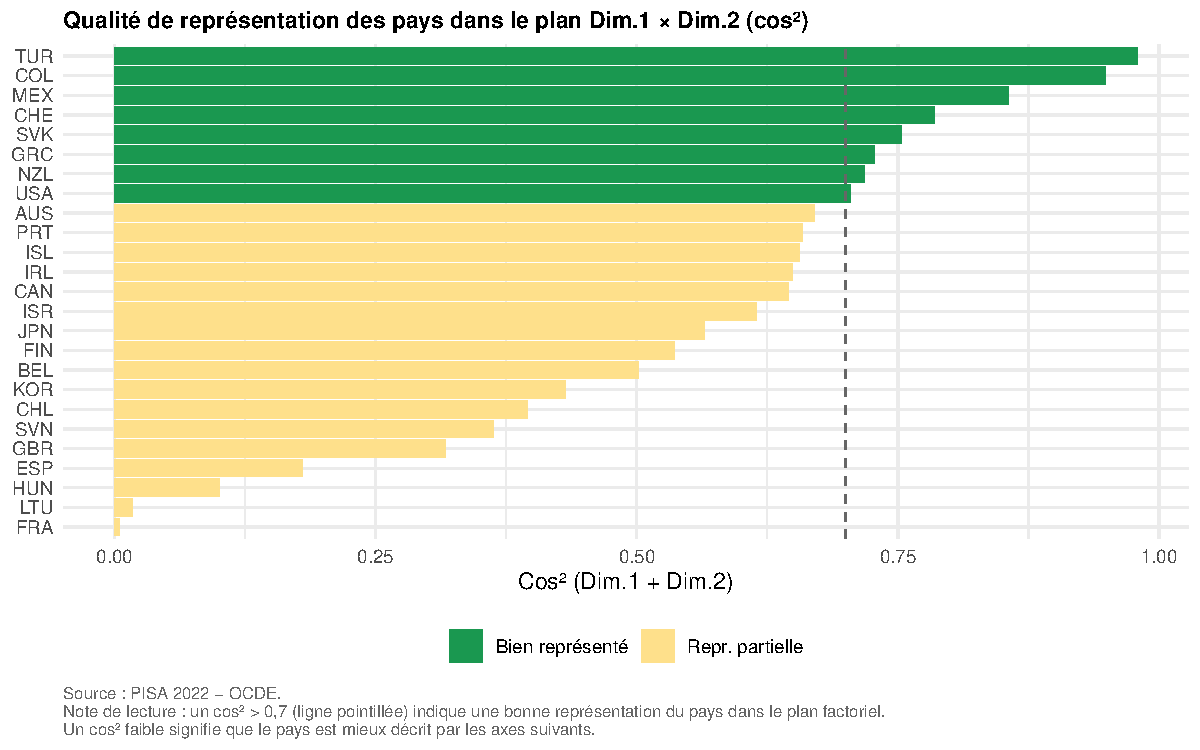
\includegraphics[keepaspectratio]{rapport_files/figure-pdf/fig-29-1.pdf}}

}

\caption{\label{fig-29}-acp-cos2}

\end{figure}%

\begin{figure}

\centering{

\pandocbounded{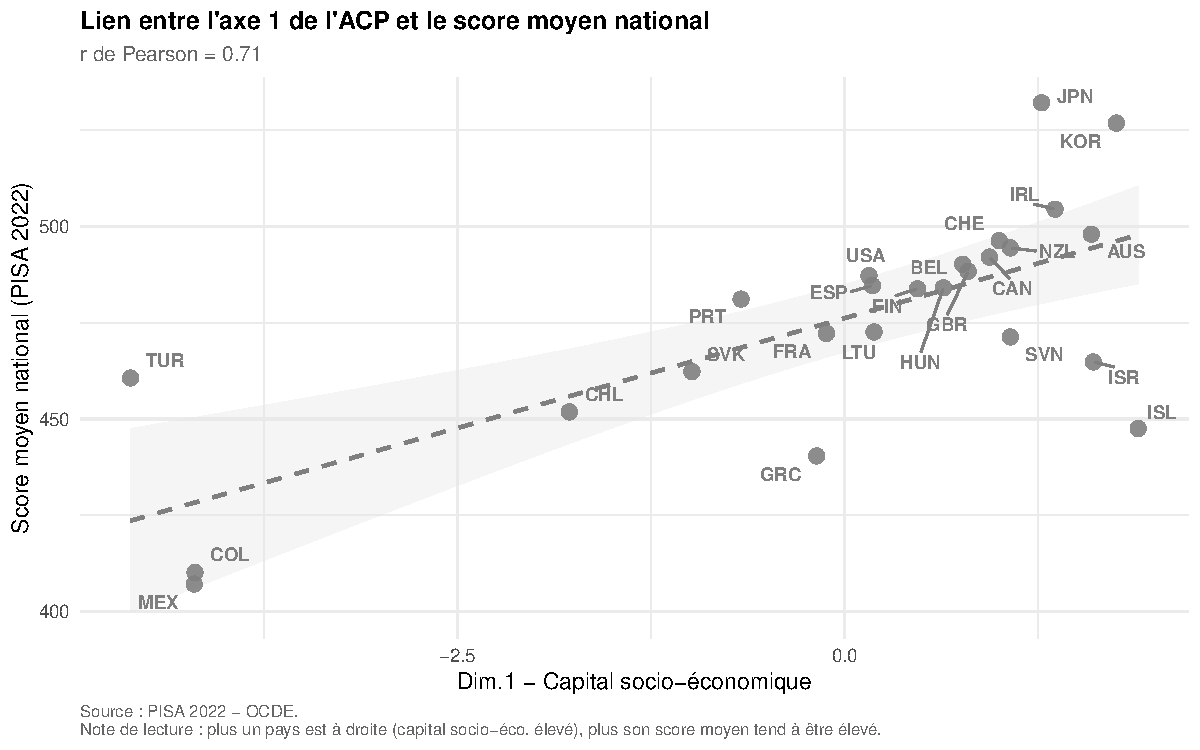
\includegraphics[keepaspectratio]{rapport_files/figure-pdf/fig-30-1.pdf}}

}

\caption{\label{fig-30}-acp-synthese}

\end{figure}%

\protect\phantomsection\label{refs}
\begin{CSLReferences}{1}{1}
\bibitem[\citeproctext]{ref-bourdieu1970reproduction}
Bourdieu, Pierre, et Jean-Claude Passeron. 1970. \emph{La Reproduction :
Éléments pour une théorie du système d'enseignement}. Les Éditions de
Minuit.

\bibitem[\citeproctext]{ref-ekole2024inegalites}
Charbonnier, Éric. 2024. \emph{Les inégalités à l'école commencent dès
le plus jeune âge et sont largement influencées par le milieu
socio-économique}.
\url{https://www.ekole.fr/blog/inegalites-ecole-commencent-des-plus-jeune-age-sont-largement-influencees-par-milieu-socio-economique-selon-ocde}.

\bibitem[\citeproctext]{ref-hanushek2006school}
Hanushek, Eric A., et Ludger Wößmann. 2006. {«~Does Educational Tracking
Affect Performance and Inequality? Differences-in-Differences Evidence
Across Countries~»}. \emph{The Economic Journal} 116 (510): C63‑76.
\url{https://doi.org/10.1111/j.1468-0297.2006.01076.x}.

\bibitem[\citeproctext]{ref-ocde2022pisa}
OCDE. 2023. \emph{PISA 2022 Results (Volume I) : The State of Learning
and Equity in Education}. OECD Publishing.
\url{https://doi.org/10.1787/53f23881-en}.

\bibitem[\citeproctext]{ref-ocde2025regards}
OCDE. 2025. \emph{Regards sur l'éducation 2025 : Indicateurs de l'OCDE}.
Éditions OCDE. \url{https://doi.org/10.1787/b26d545c-fr}.

\bibitem[\citeproctext]{ref-vp2023ocdefrance}
Vie publique. 2023. \emph{Rapport de l'OCDE sur l'éducation en France :
persistance des inégalités dans l'accès aux diplômes}.
\url{https://www.vie-publique.fr/en-bref/300175-rapport-ocde-sur-leducation-en-france-persistance-des-inegalites}.

\end{CSLReferences}




\end{document}
